% !TeX root = thesis.tex
% !TeX spellcheck = en_US
% !TeX encoding = UTF-8
\documentclass[english, LaM, oneside]{sapthesis}%remove "english" for a thesis written in Italian

%\usepackage[utf8]{inputenx}
%\usepackage{xcolor}
%\usepackage{indentfirst}
%\usepackage{microtype}

%\usepackage{lettrine}
%\linespread{0.9}

% This can be used to make space between section names more compact. The titlesec package allows changing how chapters are displayed, numerated, etc.
%\usepackage[compact]{titlesec}
% to get the bibliography in the toc
\usepackage[nottoc,notlot,notlof,chapter]{tocbibind}

\newcommand{\thesistitle}{{\sc ltl} and Past {\sc ltl} on Finite Traces for Planning and Declarative Process Mining}

\usepackage{index}
\usepackage{hyperref}
\usepackage{wrapfig}
\usepackage[round]{natbib}
\bibliographystyle{plainnat}

\usepackage[intoc,refpage]{nomencl} %refeq
\makenomenclature

%\usepackage{qtree}
% The algorithm packages have to be after hyperref.
\usepackage{algorithm}
\usepackage{algpseudocode}

\algnewcommand\algorithmicforeach{\textbf{foreach}}
\algdef{S}[FOR]{ForEach}[1]{\algorithmicforeach\ #1\ \algorithmicdo}

\usepackage{mathtools}
\usepackage{amssymb, amsmath, amsthm}
\usepackage{xspace, float, graphicx, pstricks}
%\usepackage{mathabx}

\usepackage{caption}% http://ctan.org/pkg/caption
\captionsetup[ruled]{labelsep=period}
\makeatletter
\@addtoreset{algorithm}{chapter}% algorithm counter resets every chapter
\makeatother
\renewcommand{\thealgorithm}{\thechapter.\arabic{algorithm}}% Algorithm # is <chapter>.<algorithm>

\usepackage{subcaption}
%\usepackage[autostyle]{csquotes}  
\usepackage{graphicx}
%\graphicspath{{./images/}}
\usepackage{rotating}     

\usepackage{listings}
% Custom colors
\usepackage{color}
\definecolor{deepblue}{rgb}{0,0,0.5}
\definecolor{deepred}{rgb}{0.6,0,0}
\definecolor{deepgreen}{rgb}{0,0.5,0}
\definecolor{backcolour}{rgb}{0.95,0.95,0.92}
\definecolor{codegray}{rgb}{0.5,0.5,0.5}

\usepackage{accsupp}    
\newcommand{\noncopynumber}[1]{
	\BeginAccSupp{method=escape,ActualText={}}
	#1
	\EndAccSupp{}
}
\lstdefinestyle{Python}{
	language        = Python,
	backgroundcolor=\color{backcolour},
	basicstyle      = \ttfamily,
	keywordstyle    = \color{deepblue},
	stringstyle     = \color{deepgreen},
	commentstyle    = \color{codegray}\ttfamily,
	numberstyle=\tiny\color{codegray}\noncopynumber,
	columns=flexible,
	numbers=left,
	stepnumber=1
}

\lstdefinestyle{Mona}{
	basicstyle      = \ttfamily,
	numberstyle=\tiny\color{codegray}\noncopynumber,	
	columns=flexible,
	numbers=left,
	stepnumber=1	
}

\lstdefinelanguage{PDDL}{
  basicstyle      = \ttfamily,
  sensitive=false,    % not case-sensitive
  morecomment=[l]{;}, % line comment
  alsoletter={:,-},   % consider extra characters
  numberstyle=\tiny\color{codegray}\noncopynumber,	
  numbers=left,
  stepnumber=1,
  morekeywords={
    define,domain,problem,not,and,or,when,forall,exists,either,
    :domain,:requirements,:types,:objects,:constants,
    :predicates,:action,:parameters,:precondition,:effect,
    :fluents,:primary-effect,:side-effect,:init,:goal,
    :strips,:adl,:equality,:typing,:conditional-effects,
    :negative-preconditions,:disjunctive-preconditions,
    :existential-preconditions,:universal-preconditions,:quantified-preconditions,
    :functions,assign,increase,decrease,scale-up,scale-down,
    :metric,minimize,maximize,
    :durative-actions,:duration-inequalities,:continuous-effects,
    :durative-action,:duration,:condition
  }
}
%references color
\hypersetup{
	hyperfootnotes=true,            
	bookmarks=true,         
	colorlinks=true,
	linkcolor=black, %red
	linktoc=page,
	anchorcolor=black,
	citecolor=black, %red
	urlcolor=black, %blue
	pdftitle={\thesistitle},
	pdfsubject = {Master Thesis, University of Rome ``Sapienza''},
	pdfauthor={Francesco Fuggitti},
	pdfkeywords={master thesis, sapienza, roma, university, francesco fuggitti}
	pdfauthor = {\textcopyright\ \today\ Francesco Fuggitti},
}

\theoremstyle{plain}
\newtheorem{theorem}{Theorem}[chapter] % reset theorem numbering for each chapter
\newtheorem{lemma}[theorem]{Lemma}
\theoremstyle{definition}
\newtheorem{definition}{Definition}[chapter]
\newtheorem{example}{Example}[chapter]

\newgeometry{twoside}

%opening
\title{\thesistitle}
\author{Francesco Fuggitti}
\IDnumber{1735212}
\course[override]{Master of Science in Engineering in Computer Science}
\courseorganizer{Faculty of Information Engineering, Informatics, and Statistics}
\submitdate{2017/2018}
\copyyear{2018}
\advisor{Prof. Giuseppe De Giacomo}
\authoremail{fuggitti.1735212@studenti.uniroma1.it}
\examdate{$31^{\text{st}}$ October 2018}
\examiner{Prof. Alberto Marchetti Spaccamela}
\examiner{Prof. Silvia Bonomi}
\examiner{Prof. Francesco Delli Priscoli}
\examiner{Prof. Maurizio Lenzerini}
\examiner{Prof. Daniele Nardi}
\examiner{Prof. Leonardo Querzoni}
\examiner{Prof. Marco Schaerf}    

\allowdisplaybreaks

\begin{document}
	%%%%%%%%%%%%%%%%%%%%%%%%%% General
\newcommand{\Section}[1]{Section \ref{#1}}

\newcommand{\myi}{(\emph{i})\xspace}
\newcommand{\myii}{(\emph{ii})\xspace}
\newcommand{\myiii}{(\emph{iii})\xspace}
\newcommand{\myiv}{(\emph{iv})\xspace}
\newcommand{\myv}{(\emph{v})\xspace}
\newcommand{\myvi}{(\emph{vi})\xspace}
\newcommand{\myvii}{(\emph{vii})\xspace}
\newcommand{\myviii}{(\emph{viii})\xspace}

%% general math
%\newcommand{\A}{\mathcal{A}} 
\newcommand{\B}{\mathcal{B}}
%\newcommand{\C}{\mathcal{C}} 
\newcommand{\D}{\mathcal{D}}
\newcommand{\E}{\mathcal{E}} \newcommand{\F}{\mathcal{F}}
\newcommand{\G}{\mathcal{G}} \renewcommand{\H}{\mathcal{H}}
\newcommand{\I}{\mathcal{I}} \newcommand{\J}{\mathcal{J}}
\newcommand{\K}{\mathcal{K}} \renewcommand{\L}{\mathcal{L}}
\newcommand{\M}{\mathcal{M}} \newcommand{\N}{\mathcal{N}}
\renewcommand{\O}{\mathcal{O}} \renewcommand{\P}{\mathcal{P}}
\newcommand{\Q}{\mathcal{Q}} \newcommand{\R}{\mathcal{R}}
\renewcommand{\S}{\mathcal{S}} \newcommand{\T}{\mathcal{T}}
\newcommand{\U}{\mathcal{U}} \newcommand{\V}{\mathcal{V}}
\newcommand{\W}{\mathcal{W}} \newcommand{\X}{\mathcal{X}}
\newcommand{\Y}{\mathcal{Y}} \newcommand{\Z}{\mathcal{Z}}

\newcommand{\limp}{\mathbin{\rightarrow}}
\newcommand{\ind}{\hspace*{.18in}}

\newcommand{\cla}[1]{\makebox[0pt]{\hss#1\hss}}
\newcommand{\Once}{%
  \sbox0{$\Diamond$}%
  \usebox0\kern-.5\wd0\cla{\raisebox{.1ex}{\scalebox{.7}[1]{$-$}}}\kern.5\wd0%
}

%% LTL
\newcommand{\Atom}{A}
\newcommand{\Always}{\raisebox{-0.27ex}{$\square$}}
\newcommand{\Next}{\raisebox{-0.27ex}{\LARGE$\circ$}}
\newcommand{\Wnext}{\raisebox{-0.27ex}{\LARGE$\bullet$}}
\newcommand{\lUntil}{\mathop{\U}}
\newcommand{\Yesterday}{\raisebox{-0.27ex}{$\ominus$}}
\newcommand{\Since}{\mathop{\S}}
\newcommand{\Release}{\mathop{\R}}
\newcommand{\Wuntil}{\mathop{\W}}
\newcommand{\true}{\mathit{true}}
\newcommand{\final}{\mathit{Final}}
\newcommand{\false}{\mathit{false}}
\newcommand{\ttrue}{{\mathit{tt}}}
\newcommand{\ffalse}{\mathit{ff}}
\newcommand{\Last}{\mathit{Last}}
\newcommand{\Ended}{\mathit{End}}
\newcommand{\length}{\mathit{length}}
\newcommand{\last}{\mathit{last}}
\newcommand{\End}{\mathit{end}}
\newcommand{\nnf}{\mathit{nnf}}
\newcommand{\BOX}[1]{ [#1]}
\newcommand{\DIAM}[1]{\langle #1 \rangle}
\newcommand{\transl}{f}


%% Logics
\newcommand{\LT}{{\sc lt}$_f$\xspace}
\newcommand{\LTi}{{\sc lt}$_i$\xspace}
\newcommand{\PLTL}{{\sc pltl}\xspace}
\newcommand{\FLTL}{{\sc \$fltl}\xspace}
\newcommand{\FstarLTL}{{\sc \$$^*$fltl}\xspace}
\newcommand{\PL}{{\sc pl}\xspace}
\newcommand{\LTL}{{\sc ltl}\xspace}
\newcommand{\LTLf}{{\sc ltl}$_f$\xspace}
\newcommand{\PLTLf}{{\sc pltl}$_f$\xspace}
\newcommand{\LTLp}{{\sc ltl}p$_f$\xspace}
\newcommand{\LDL}{{\sc ldl}\xspace}
\newcommand{\LDLf}{{\sc ldl}$_f$\xspace}
\newcommand{\RE}{{\sc re}$_f$\xspace}
\newcommand{\REGEX}{{\sc re}\xspace}
\newcommand{\DL}{{\sc dl}\xspace}
\newcommand{\PDL}{{\sc pdl}\xspace}
\newcommand{\PDDL}{{\sc pddl}\xspace}
\newcommand{\FOND}{{\sc fond}\xspace}
\newcommand{\FOf}{{\sc fo}$_f$\xspace}
\newcommand{\MSOf}{{\sc mso}$_f$\xspace}
\newcommand{\FO}{{\sc fo}\xspace}
\newcommand{\FOL}{{\sc fol}\xspace}
\newcommand{\MSO}{{\sc mso}\xspace}
%\newcommand{\ATA}{{\sc ata}\xspace}
\newcommand{\AFW}{{\sc afw}\xspace}
\newcommand{\NFA}{{\sc nfa}\xspace}
\newcommand{\DFA}{{\sc dfa}\xspace}
\newcommand{\DFAs}{{\sc dfa}s\xspace}
\newcommand{\GTAs}{{\sc gta}s\xspace}
\newcommand{\declare}{{\sc declare}\xspace}
\newcommand{\wsos}{{\sc ws1s}\xspace}
\newcommand{\wsts}{{\sc ws2s}\xspace}
\newcommand{\bdds}{{\sc bdd}s\xspace}
\newcommand{\bdd}{{\sc bdd}\xspace}
\newcommand{\mls}{{\sc m2l-s}tr\xspace}
\newcommand{\fol}{\mathit{fol}}
\newcommand{\folp}{\mathit{fol_p}}
\newcommand{\f}{\mathit{f}}
%\newcommand{\g}{\mathit{g}}
\newcommand{\re}{\mathit{re}}


\newcommand{\tup}[1]{\langle #1 \rangle}

\newcommand{\Stop}{\mathit{stop}}
\newcommand{\rew}{\mathit{rew}}
\newcommand{\Tr}{\mathit{Tr}}

\newcommand{\LOGSPACE}{{\sc logspace}\xspace}
\newcommand{\NLOGSPACE}{{\sc nlogspace}\xspace}
\newcommand{\PTIME}{{\sc ptime}\xspace}
\newcommand{\NP}{{\sc np}\xspace}
\newcommand{\EXPTIME}{{\sc exptime}\xspace}
\newcommand{\PSPACE}{{\sc pspace}\xspace}
\newcommand{\TWOEXPTIME}{{\sc 2exptime}\xspace}


\newcommand{\expand}{\textbf{\textit{E}}}
\newcommand{\ttt}{{\textbf{\textit{T}}}}
\newcommand{\fff}{{\textbf{\textit{\texttt{F}}}}}

\newcommand{\fstate}{s_f}

\newcommand{\atomize}[1]{\texttt{"}\ensuremath{#1}\texttt{"}}


% misc
\newcommand{\MONA}{{\sc mona}\xspace}
\newcommand{\FLLOAT}{{\sc flloat}\xspace}
\newcommand{\suc}{\textit{succ}\xspace}
\newcommand{\pre}{\textit{prev}\xspace}
\newcommand{\folInter}{$\I = (\Delta^I,\cdot^{\I})$\xspace}
\newcommand{\rcon}{RCon}
\newcommand{\janus}{{\sc janus}\xspace}

%RL
\newcommand{\MDP}{\M}
\newcommand{\States}{S}
\newcommand{\Actions}{A}
\newcommand{\TrFun}{T}
\newcommand{\Reward}{R}
\newcommand{\DiscFact}{\gamma}
\newcommand{\Policy}{\rho}
\newcommand{\ExpRet}{G}
\newcommand{\ValFun}{v}
\newcommand{\qFun}{q}

\newcommand{\ValOptFun}{\ValFun^*}
\newcommand{\qOptFun}{\qFun^*}
\newcommand{\OptPolicy}{\Policy^*}

\newcommand{\ValFunEst}{V}
\newcommand{\qFunEst}{Q}
\newcommand{\LRate}{\alpha}

\newcommand{\NMRDP}{\N}
\newcommand{\NMReward}{\bar{\Reward}}
\newcommand{\NMPolicy}{\bar{\Policy}}

\newcommand{\traj}{\tup{s_0, a_0, \dots, s_{n-1}, a_{n-1}, s_n}}
\newcommand{\trajprime}{\tup{s'_0, a_0, \dots, s'_{n-1}, a_{n-1}, s'_n}}
\newcommand{\projtraj}{\tup{s_0, s_1, \dots, s_n}}
\newcommand{\projtrajprime}{\tup{s'_0, s'_1, \dots, s'_n}}

\newcommand{\MDPagent}{\MDP_{ag}}
\newcommand{\TrFunAgentGoal}{\TrFun_{ag}^{g}}

\newcommand{\bqs}{\mathbf{q}}

%LOGIC

\newcommand{\Prop}{\P}
\newcommand{\PropInt}{\Pi}
\newcommand{\PropFormula}{\phi}
\newcommand{\trace}{\pi}
\newcommand{\Kripke}{\K}
\newcommand{\tm}[1]{\ \text{#1}\ }
\newcommand{\tiff}{\tm{iff}}
\newcommand{\DECLARE}{{\sc declare}\xspace}


\newcommand{\automaton}{\mathcal{A}}
\newcommand{\LLf}{\LTLf/\LDLf}
\newcommand{\DfunSym}{\partial}
\newcommand{\Dfun}[1]{\DfunSym\lparen #1,\PropInt \rparen}
\newcommand{\DfunEps}[1]{\DfunSym\lparen #1, \epsilon\rparen}
\newcommand{\lAND}{\wedge}
\newcommand{\lOR}{\vee}
\newcommand{\NOT}{\lnot}
\newcommand{\regexp}{\varrho}
\newcommand{\TrueDelta}[1]{\textit{\textbf{\texttt{T}}}_{#1}}
\newcommand{\FalseDelta}[1]{\textit{\textbf{\texttt{F}}}_{#1}}
\newcommand{\bOne}{\mathbf{1}}
\newcommand{\bZero}{\mathbf{0}}
\newcommand{\LTS}{{\sc lts}\xspace}
\newcommand{\LDLfToNFA}{{\sc ldl}$_f2$\NFA}
\newcommand{\LDLfToDFA}{{\sc ldl}$_f2$\DFA}
\newcommand{\LTLfToDFA}{{\sc ltl}$_f2$\DFA}
\newcommand{\PLTLToDFA}{{\sc pltl}$2$\DFA}
\newcommand{\LTLfToFOL}{{\sc ltl}$_f2$\FOL}
\newcommand{\PLTLToFOL}{{\sc pltl}$2$\FOL}

\newcommand{\Sapientino}{{\sc sapientino}\xspace}
\newcommand{\Breakout}{{\sc breakout}\xspace}
\newcommand{\Minecraft}{{\sc minecraft}\xspace}

%math

\newcommand{\set}[1]{\{#1\}}
\newcommand{\Naturals}{\mathbb{N}}
\newcommand{\Reals}{\mathbb{R}}
\newcommand{\defeq}{\coloneqq}


%algpseudocode
\algnewcommand\algInput{\textbf{input}}
\algnewcommand\algOutput{\textbf{output}}


%%% Local Variables:
%%% mode: latex
%%% TeX-master: "main"
%%% save-place: t
%%% End:

	
	\frontmatter	
	\maketitle
	
\begin{abstract}
The application of \LTL and Past \LTL on Finite Traces is of particular interest for different fields in Artificial Intelligence (AI) and Computer Science (CS). In this thesis, we focus on the application of these two formal languages to Planning and Declarative Process Mining. For this purpose, the design and implementation of the \LTLfToDFA framework has been crucial to the application of \LTLf and \PLTL in both research fields. In Planning, we direct our attention to \FOND planning for \LTLf and \PLTL goals showing a new encoding of those temporal goals in standard \PDDL. We formally provide experimental evidence that it is possible to restrict the manner used by the plan to reach the goal specified in future and past modalities. With respect to Declarative Process Mining, we generalize the Janus approach for computing the interestingness of traces out of event logs, giving a new representation of the constraint formula allowing propositional formulas as activation condition.
\end{abstract}
	

	
	\tableofcontents
%	\listoffigures
%	\listoftables
	
	\mainmatter
	\chapter{Introduction}
\section{Context}
The literature on Artificial Intelligence (AI) and Computer Science (CS) has directed attention to Linear Temporal Logic (\LTL) as the formal language for temporal specification of the sequence of actions of an agent or a system of agents \citep{fagin2004reasoning}. Initially, \LTL on infinite traces was formulated in Computer Science as a specification language for concurrent programs \citep{Pnueli:1977:TLP:1382431.1382534}.

More specifically, the variant of \LTL evaluated on \textit{finite} traces (\LTLf) and its past counterpart  Past \LTL (\PLTL), treated in this thesis, have been thoroughly investigated in \cite{de2013linear,lichtenstein1985glory}. Concerning \LTLf, \cite{de2013linear} conceptualise the encoding of \LTLf to First-Order Logic (\FOL) by defining the translation function $fol(\varphi, x)$. \cite{zpv2018} adopts this function, but modifying it with the appropriate built-in operators of \MONA. \MONA was formerly applied in \cite{zhu2017symbolic} because of its performativity. Regarding \PLTL temporal specification, formerly studied in ``The Glory of the Past'' \citep{lichtenstein1985glory}, \cite{zpv2018} formulates the translation function $fol_p(\varphi, x)$ allowing the encoding of \PLTL to \FOL through the application of \MONA operators. Nevertheless, afore-mentioned researches have not yet implemented such a translation function with the \MONA tool starting directly from a \PLTL formula. 
%tool capable of generating Deterministic Finite-state Automata (\DFA) taking advantage of the \MONA tool.

The above-mentioned formal languages, \LTLf and \PLTL, are mechanism for specifying temporally extended goals in Planning and formula constraints in Business Process Modeling (BPM), more specifically in Declarative Process Mining. While \cite{camacho2017non} analyse non-deterministic planning for \LTL on finite and infinite traces goals, academics have not investigated planning for \PLTL goals. Regarding BPM, \cite{cecconi2018interestingness}, by employing the augmentation of \LTLf with past modalities, introduce a new approach to compute the ratio between the number of times a constraint formula is satisfied by a trace and the number of times the former is activated by the latter. However, such an approach conceptualises the activation condition of the constraint as a single task and it can only handle \declare constraints, under a practical perspective.

In the next Section, we are going to formulate the objectives of the thesis by explaining issues pertaining to the applications of \LTLf and \PLTL, particularly, in Planning and BPM.
\section{Objectives}
This thesis sets specific objectives about the definition and application of \LTLf and \PLTL formalisms by referring to problems on cited research works.

Firstly, even though \cite{de2013linear} formalized the theory behind the translation from an \LTLf formula to \FOL and \cite{zpv2018} retrieved this approach customizing it for \MONA, they have not yet implemented the translation functions both for \LTLf and \PLTL employing the \MONA tool for the generation of the symbolic Deterministic Finite-state Automaton (\DFA). Such an implementation is critical for the optimization of the conversion processes of \LTLf and \PLTL formulas to \DFA as shown in \cite{zhu2017symbolic}. Therefore, the thesis will build a tool, named \LTLfToDFA, which will use \MONA to convert both \LTLf and \PLTL formulas to their corresponding \DFA.

Secondly, to the best of our knowledge, the literature on AI has not yet investigated planning for \PLTL goals. The investigation on planning for \PLTL goals is of paramount importance in one respect. It generalizes the restriction of modes used by the plan to reach the goal. While previous works \citep{camacho2017non, camacho2018finite, camacho2018ltl} considered future goal specifications (i.e. using \LTLf goals), the objective of this thesis is not only to allow past goal specifications (i.e. using \PLTL goals), but also to provide a new formalization of those temporally extended goals in the Planning Domain Definition Language (\PDDL). Such an objective will be attained through the result given by the \LTLfToDFA tool.

Finally, the thesis will propose a generalization of the Janus approach firstly introduced in \cite{cecconi2018interestingness}, under a theoretical and practical perspective. The Janus approach has two main drawbacks. In particular, the activation condition of a constraint formula could only be specified as a single task, since \cite{cecconi2018interestingness} take into account only \declare constraints, thoroughly investigated in \cite{pesic2008constraint}. As a result, the constraint can be activated if, at a certain instant of the trace, one and only one task is executed. Secondly, the original Janus algorithm implementation does not include a tool to directly convert any \LTLf and \PLTL formulas into their related \DFAs. The thesis will address such limitations by devising a generalization of the Janus approach, allowing any type of constraint and, then, employing the \LTLfToDFA tool to directly generate \DFA of any \LTLf and \PLTL formulas.
\section{Results}
The thesis significantly contributes to the research areas of Formal Methods, Planning and Business Process Modeling. 

In the first place, by directing attention to the interpretation of \LTL and \PLTL on \textit{finite} traces, we designed and implemented a new tool, called \LTLfToDFA, that translates any \LTLf/\PLTL formula to a Deterministic Finite-state Automaton (\DFA). \textsc{ltl}$_f2$\textsc{dfa} is relevant in two respects. It is the first tool able to directly convert both \textsc{ltl}$_f$ and \textsc{pltl} formulas to their corresponding \textsc{dfa}. Secondly, it adopts the \textsc{mona} tool for the generation of automata. Accordingly, we have advanced researches in \cite{zhu2017symbolic,zpv2018}, by delivering the \LTLfToDFA software package. Moreover, the \LTLfToDFA is also available on \href{http://ltlf2dfa.diag.uniroma1.it}{http://ltlf2dfa.diag.uniroma1.it}.

In the second place, concerning Planning, we have explored how \textsc{ltl}$_f$ and \textsc{pltl} can be used for expressing extended temporal goals in fully observable \textit{non-deterministic} (\textsc{fond}) planning problems. In these terms, we have proposed a new approach in compiling temporally extended goals together with the original planning domain, specified in \textsc{pddl}, which is suitable for input to standard (\textsc{fond}) planners (e.g. FOND-SAT planner in \cite{geffner2018compact}).
The encoding of those temporal goals, directly in the \textsc{pddl} domain and problem, relies on the result given by \textsc{ltl}$_f2$\textsc{dfa}. More specifically, we have encoded \textsc{dfa} transitions as a new \textsc{pddl} operator and modified the goal accordingly. The absolute novelty is that, given the new \textsc{ltl}$_f2$\textsc{dfa} tool, it is now possible to express temporal extended goals not only in \textsc{ltl}$_f$, but also in \textsc{pltl} (i.e. with past modalities), unlike  former researches in this area of application \citep{camacho2017non, camacho2018finite, camacho2018ltl}.

In the third place, regarding \textsc{BPM}, \textsc{ltl}$_f2$\textsc{dfa} enables the extension and generalization of the Janus approach in declarative process mining for computing the \textit{interestingness degree} of traces in event logs. From a theoretical perspective, we have generalized the Janus approach by giving a new representation of the constraint formula allowing propositional formulas as activation condition, rather than a single task as in \cite{cecconi2018interestingness}. From a practical perspective, we have implemented this modified approach by exploiting the power of the \textsc{ltl}$_f2$\textsc{dfa} tool. In such a scenario, \textsc{ltl}$_f2$\textsc{dfa} has allowed to generate, at execution time, \textsc{dfa}s for any type of formula, overcoming the original limitation of the Janus approach to \textsc{declare} constraints.
\section{Structure of the Thesis}
The thesis is structured as follows:
\begin{itemize}
\item In Chapter \ref{ch:theory}, we will illustrate the theoretical framework, consisting of \LTL, \LTLf and \PLTL formalisms, underlying the thesis. These formal languages will be described focusing the attention on their syntax, semantics and interesting properties. Besides, we will be talking about the theory behind the translation procedure of \LTLf and \PLTL formulas to \DFAs. Finally, we will present the \MONA tool explaining in details the encoding process starting from an \LTLf/\PLTL formula to a \MONA program passing through a \FOL translation.

\item In Chapter \ref{ch:ltlf2dfa}, we will present the \LTLfToDFA Python package. We will also describe the structure of the package, discussing in detail its implementation highlighting all the main features and, finally, seeing how it performs in time relatively to the \FLLOAT Python package.

\item In Chapter \ref{ch:planning}, we will face the problem of \FOND Planning for \LTLf/\PLTL goals. In particular, we will propose a new solution, called \FONDFOR, that essentially reduces the problem to a ``classical'' \FOND planning problem. This will be possible thanks to our \LTLfToDFA Python tool which will be employed for the encoding of temporally extended goals into standard \PDDL. Then, we will also described in details the \FONDFOR implementation, highlighting all its main features. Finally, we will see examples of execution results.

\item In Chapter \ref{ch:janus}, we will present how the \LTLfToDFA Python package has been well employed in the field of Business Process Management. In particular, we will explore the Janus approach to declarative process mining enhancing its peculiarities and, at the same time, giving our substantial contributions in generalizing the approach itself. After that, we will describe the implementation of the \janus algorithm, modified accordingly, highlighting all its main features. Finally, we will see examples of execution results.

\item In Chapter \ref{ch:conclusion}, the thesis will conclude summarizing its main achievements and discussing possible future works.
\end{itemize}
























	\chapter{\PLTL and \LTLf}
This chapter will deal with the theoretical framework on which all topics present in the thesis are based. Initially, we will introduce the widely known Linear-Time Temporal Logic (\LTL) and the Past Linear Time Temporal Logic (\PLTL), focusing on their syntax and semantic. Secondly, we will talk about the concept of \textit{Finite Trace} in these formal languages and how it changes them. Specifically, we will describe the Linear Time Temporal Logic over Finite Traces (\LTLf). Then, we will illustrate the theory behind the transformation of an \LTLf or \PLTL formula to a Deterministic Finite State Automaton (\DFA). Finally, we will describe the translation of an \LTLf or \PLTL formula to the classic First-Order Logic formalism (\FOL) and the translation of a \FOL formula into a program that the \MONA, a tool that translates formulas into a \DFA, can manage. Some examples will be provided, but we will suppose the reader to be confident with classical logic and automata theory.
\section{Linear Temporal Logic (\LTL)}
\textit{Temporal Logic} formalisms are a set of formal languages designed for representing temporal information and reasoning about time within a logical framework \citep{sep-logic-temporal}. Indeed, these logics are used when propositions have their truth value dependent on time. Hence, this kind of formal languages are able to specify properties about how a system changes over time.

In this scenario, we find the \textit{Linear Temporal Logic} (\LTL) \citep{Pnueli:1977:TLP:1382431.1382534} which is a modal temporal logic with modalities referring to time. \LTL is a very well known temporal logic since it has been extensively used in AI and CS. For instance, it has been employed in planning, reasoning about actions, declarative process mining and verification of software/hardware systems.
\subsection{Syntax}
Given a set of propositional symbols $\P$, a valid \LTL formula $\varphi$ is defined as follows:
\[\begin{array}{rcl}
\varphi &::=& \top \mid \bot \mid a \mid \lnot \varphi \mid \varphi_1\land \varphi_2 \mid \Next\varphi \mid \varphi_1 \lUntil \varphi_2
\end{array}
\]
where $a\in \P$. The unary operator \Next  (\emph{next-time}) and the binary operator $\lUntil$  (\emph{until}) are temporal operators and we use $\top$ and $\bot$ to denote $\true$ and $\false$ respectively. Moreover, all classical logic operators $\lOR, \Rightarrow, \Leftrightarrow$ can be used. 
Intuitively, \Next $\varphi$ says that $\varphi$ is true at the \textit{next} instant, $\varphi_1 \lUntil \varphi_2$ says that at some future instant, $\varphi_2$ will hold and \textit{until} that point $\varphi_1$ holds. We also define common abbreviations for some specific temporal formulas: \emph{eventually} as $\Diamond \varphi \doteq \true \lUntil \varphi$, \emph{always} as $\Box \varphi \doteq \lnot \Diamond \lnot \varphi$, \emph{weak-next} as $\W \doteq \lnot \Next \lnot \varphi$ and \emph{release} as $\varphi_1 \Release \varphi_2 \doteq \lnot (\lnot \varphi_1 \lUntil \lnot \varphi_2)$. 

\LTL allows to express a lot of interesting properties defined over time. In the Example \ref{ltl-formula-examples} we show some of them.
\begin{example}\label{ltl-formula-examples}
Interesting \LTL patterns:
\begin{itemize}
	\item \emph{Safety}: $\Box \lnot \varphi$, which means "it is always true that property in $\varphi$ will never happen" or "something bad will not happen". For instance, $\Box \lnot (reactor-temp > 1000)$ (the temperature of the reactor must never be over 1000).
	\item \emph{Liveness}: $\Diamond \varphi$, which means "sooner or later $\varphi$ will hold" or "something good will happen". For instance, $\Diamond rich$ (eventually I will become rich).
	\item \emph{Strong fairness}: $\Box \Diamond \varphi_1 \Rightarrow \Box \Diamond \varphi_2$, "if something is attempted/requested infinitely often, then it will be successful/allocated infinitely often". For instance, $\Box \Diamond ready \Rightarrow \Box \Diamond run$ (if a process is in ready state infinitely often, then it will be selected by the scheduler infinitely often).
\end{itemize}
\end{example}
\subsection{Semantics}
The semantics of the main operators of \LTL over \textit{infinite traces} are expressed as an $\omega$-word over the alphabet $2^\P$. We give the following definitions:
\begin{definition}\label{ltl-semantics}
	Given an infinite trace $\trace$, we inductively define when an \LTL formula $\varphi$ is $true$ at an instant $i$, in symbols $\trace, i \models \varphi$, as follows:
	\begin{align*}
	\trace, i &\models a, \tm{for} a\in\P \tiff a \in \trace(i)\\
	\trace, i &\models \lnot \varphi \tiff \trace, i \not\models \varphi\\
	\trace, i &\models \varphi_1 \lAND \varphi_2 \tiff \trace, i \models \varphi_1 \lAND \trace, i \models \varphi_2\\
	\trace, i &\models \Next\varphi \tiff \trace,i+1 \models \varphi\\
	\trace, i &\models \varphi_1 \lUntil \varphi_2 \tiff \exists j. (j\ge i) \lAND \trace,j \models \varphi_2 \lAND\forall k. (i\le k < j) \Rightarrow \trace, k \models \varphi_1\\
	\end{align*}
\end{definition}
\begin{definition}\label{ltl-sat-val-ent}
An \LTL formula $\varphi$ is \emph{true} in $\trace$, in notation $\trace \models \varphi$, if $\trace, 0 \models \varphi$. A formula $\varphi$ is \emph{satisfiable} if it is true in some $\trace$ and is \emph{valid} if it is true in every $\trace$. A formula $\varphi_1$ logically implies another formula $\varphi_2$, in symbols $\varphi_1 \models \varphi_2 \tiff \forall \trace, \trace \models \varphi_1 \Rightarrow \trace \models \varphi_2$.
\end{definition}
Notice that satisfiability, validity and logical implication are all mutually reducible one to each other.
\begin{example}\label{ltl-sat-examples}
Validity and logical implication as satisfiability
\begin{itemize}
\item $\varphi$ is valid $\tiff \lnot \varphi$ is unsatisfiable.
\item $\varphi_1 \models \varphi_2 \tiff \varphi_1 \lAND \lnot \varphi_2$ is unsatisfiable.
\end{itemize}
\end{example}
Finally, we can state the following fundamental theorem:
\begin{theorem}[\cite{Sistla:1985:CPL:3828.3837}]
Satisfiability, validity, and logical implication for \LTL formulas are \PSPACE-complete.
\end{theorem}
\section{Linear Temporal Logic on Finite Traces (\LTLf)}
\section{Past Linear Temporal Logic (\PLTL)}
\section{\LTLfToDFA}
talk about theory behind conversion to automata in future
\section{\PLTLToDFA}
talk about theory behind conversion to automata in past
\section{\LTLfToFOL and \MONA}
talk about theory behind translation and intro with mona future
\section{\PLTLToFOL and \MONA}
talk about theory behind translation and intro with mona past

	\chapter{\LTLfToDFA}\label{ch:ltlf2dfa}
In this chapter we will present \href{https://github.com/Francesco17/LTLf2DFA}{\LTLfToDFA}, a software package  written in Python. 

\section{Introduction}\label{sec:intro}
\LTLfToDFA is a Python tool that processes a given \LTLf formula (with past and future operators) and generates the corresponding minimized \DFA using \MONA\citep{mona1998}. In addition, it offers the possibility to compute the \DFA with or without the \declare assumption \citep{DeGiacomo:2014:RLF:2893873.2894033}.
The main features provided by the library are:
\begin{itemize}
\item parsing an \LTLf formula with past or future operators;
\item translation of an \LTLf formula to \MONA program;
\item conversion of an \LTLf formula to \DFA automaton.
\end{itemize}
\LTLfToDFA can be used with Python>=3.6 and has the following dependencies:
\begin{itemize}
\item \href{http://www.dabeaz.com/ply/ply.html}{PLY}, a pure-Python implementation of the popular compiler construction tools \href{http://dinosaur.compilertools.net/}{Lex and Yacc}. It has been employed for parsing the input \LTLf formula;
\item \href{http://www.brics.dk/mona/}{\MONA}, a C++ tool that translates formulas to \DFA. It has been used for the generation of the \DFA;
\item \href{https://pypi.org/project/dotpy/}{Dotpy}, a Python library able to parse and modify \texttt{.dot} files. It has been utilized for post-processing the \MONA output.
\end{itemize}
The package is available to download on \href{https://pypi.org/project/ltlf2dfa/}{PyPI} and you can install it by typing in the terminal:
\begin{lstlisting}[language=bash]
pip install ltlf2dfa
\end{lstlisting}
All the code is available online on GitHub\footnote{https://github.com/Francesco17/LTLf2DFA}, it is open source and it is released under the \href{https://github.com/Francesco17/LTLf2DFA/blob/master/LICENSE}{MIT License}.
Moreover, \LTLfToDFA can also be tried online at \href{ltlf2dfa.diag.uniroma1.it}{ltlf2dfa.diag.uniroma1.it}.
\section{Package Structure}
The structure of the \LTLfToDFA package is quite simple. It consists of a main folder called \texttt{ltlf2dfa/} which hosts the most important library's modules:
\begin{itemize}
\item \texttt{Lexer.py}, where the Lexer class is defined;
\item \texttt{Parser.py}, where the Parser class is defined;
\item \texttt{Translator.py}, where the main APIs for the translation are defined;
\item \texttt{DotHandler.py}, where we the \MONA output is post-processed.
\end{itemize}
In the following paragraphs we will explore each module in detail.
\subsection{Lexer.py}
In the \texttt{Lexer.py} module we can find the declaration of the \texttt{MyLexer} class which is in charge of handling the input string and tokenizing it. Indeed, it implements a tokenizer that splits the input string into declared individual tokens.
To our extent, we have defined the class as in Listing \ref{code:ltlf2dfa-lexer}
\begin{lstlisting}[language=Python, style=Python, escapechar = £, label={code:ltlf2dfa-lexer}, caption={\texttt{Lexer.py} module}]
import ply.lex as lex

class MyLexer(object):

    reserved = {
        'true':     'TRUE',
        'false':    'FALSE',
        'X':        'NEXT',
        'U':        'UNTIL',
        'E':        'EVENTUALLY',
        'G':        'GLOBALLY',
        'Y':        'PASTNEXT', #PREVIOUS
        'S':        'PASTUNTIL', #SINCE
        'O':        'PASTEVENTUALLY', #ONCE
        'H':        'PASTGLOBALLY'
    }
    # List of token names.   This is always required
    tokens = (
        'TERM',
        'NOT',
        'AND',
        'OR',
        'IMPLIES',
        'DIMPLIES',
        'LPAR',
        'RPAR'
    ) + tuple(reserved.values())

    # Regular expression rules for simple tokens
    t_TRUE = r'T'
    t_FALSE = r'F'
    t_AND = r'\&'
    t_OR = r'\|'
    t_IMPLIES = r'\->'
    t_DIMPLIES = r'\<->'
    t_NOT = r'\~'
    t_LPAR = r'\('
    t_RPAR = r'\)'
    # FUTURE OPERATORS
    t_NEXT = r'X'
    t_UNTIL = r'U'
    t_EVENTUALLY = r'E'
    t_GLOBALLY = r'G'
    # PAST OPERATOR
    t_PASTNEXT = r'Y'
    t_PASTUNTIL = r'S'
    t_PASTEVENTUALLY = r'O'
    t_PASTGLOBALLY = r'H'

    t_ignore = r' '+'\n'

    def t_TERM(self, t):£\label{line:lexer-term}£
        r'[a-z]+'
        t.type = MyLexer.reserved.get(t.value, 'TERM')
        return t  # Check for reserved words

    def t_error(self, t):
        print("Illegal character '%s' in the input formula" % t.value[0])
        t.lexer.skip(1)

    # Build the lexer
    def build(self,**kwargs):
        self.lexer = lex.lex(module=self, **kwargs)
\end{lstlisting}
Firstly, we have defined the reserved words within a dictionary so to match each reserved word with its identifier.
Secondly, we have defined the tokens list with all possible tokens that can be produced by the lexer. This tokens list is always required for the implementation of a lexer.
Then, each token has to be specified by writing a regular expression rule. If the token is simple it can be specified using only a string. Otherwise, for non trivial tokens we have to write the regular expression in a class method as for our token \texttt{TERM} in line \ref{line:lexer-term}. In that case, defining the token rule as a method is also useful when we would like to perform other actions. After that, we have a method to handle unrecognized tokens and, finally, we have written the function that builds the lexer.
\subsection{Parser.py}
In the \texttt{Parser.py} module we can find the declaration of \texttt{MyParser} class which implements the parsing component of \texttt{PLY}. The \texttt{MyParser} class operates after the Lexer has split the input string into known tokens. The main feature of the parser is to interpret and build the appropriate data structure for the given input. To this extent, the most important aspect of a parser is the definition of the \textit{syntax}, usually specified in terms of a BNF\footnote{The Backus–Naur form is a notation technique for context-free grammars.} grammar, that should be unambiguous. Furthermore, \texttt{Yacc}, the parsing component of \texttt{PLY}, implements a parsing technique known as LR-parsing or shift-reduce parsing. In particular, this parsing technique works on a bottom up fashion that tries to recognize the right-hand-side of various grammar rules. Whenever a valid right-hand-side is found in the input, the appropriate action code is triggered and the grammar symbols are replaced by the grammar symbol on the left-hand-side and so on until there is no more rule to apply. The parser implementation is shown in Listing \ref{code:ltlf2dfa-parser}
\begin{lstlisting}[language=Python, style=Python, label={code:ltlf2dfa-parser}, caption={\texttt{Parser.py} module}]
import ply.yacc as yacc
from ltlf2dfa.Lexer import MyLexer

class MyParser(object):

    def __init__(self):
        self.lexer = MyLexer()
        self.lexer.build()
        self.tokens = self.lexer.tokens
        self.parser = yacc.yacc(module=self)
        self.precedence = (

            ('nonassoc', 'LPAR', 'RPAR'),
            ('left', 'AND', 'OR', 'IMPLIES', 'DIMPLIES', 'UNTIL', \
             'PASTUNTIL'),
            ('right', 'NEXT', 'EVENTUALLY', 'GLOBALLY', \
            'PASTNEXT', 'PASTEVENTUALLY', 'PASTGLOBALLY'),
            ('right', 'NOT')
        )

    def __call__(self, s, **kwargs):
        return self.parser.parse(s, lexer=self.lexer.lexer)

    def p_formula(self, p):
        '''
        formula : formula AND formula
                 | formula OR formula
                 | formula IMPLIES formula
                 | formula DIMPLIES formula
                 | formula UNTIL formula
                 | formula PASTUNTIL formula
                 | NEXT formula
                 | EVENTUALLY formula
                 | GLOBALLY formula
                 | PASTNEXT formula
                 | PASTEVENTUALLY formula
                 | PASTGLOBALLY formula
                 | NOT formula
                 | TRUE
                 | FALSE
                 | TERM
        '''

        if len(p) == 2: p[0] = p[1]
        elif len(p) == 3:
            if p[1] == 'E': # E(a) == true UNITL A
                p[0] = ('U','T', p[2])
            elif p[1] == 'G': # G(a) == not(eventually (not A))
                p[0] = ('~',('U', 'T', ('~',p[2])))
            elif p[1] == 'O': # O(a) = true SINCE A
                p[0] = ('S','T', p[2])
            elif p[1] == 'H': # H(a) == not(pasteventually(not A))
                p[0] = ('~',('S', 'T', ('~',p[2])))
            else:
                p[0] = (p[1], p[2])
        elif len(p) == 4:
            if p[2] == '->':
                p[0] = ('|', ('~', p[1]), p[3])
            elif p[2] == '<->':
                p[0] = ('&', ('|', ('~', p[1]), p[3]), ('|', ('~', p[3]),\
                p[1]))
            else:
                p[0] = (p[2],p[1],p[3])
        else: raise ValueError


    def p_expr_group(self, p):
        '''
        formula : LPAR formula RPAR
        '''
        p[0] = p[2]

    def p_error(self, p):
        raise ValueError("Syntax error in input! %s" %str(p))
\end{lstlisting}
As we can see, as soon as the parser is instantiated it builds the lexer, gets the tokens and defines their precedence if needed. Then, we have defined methods of the \texttt{MyParser} class that are in charge of constructing the syntax tree structure from tokens found by the lexer in the input string. In our case, we have chosen to use as data structure a tuple of tuples as it is the one of the simplest data structure in Python. In general, a tuple of tuples represents a tree where each node represents an item present in the formula.

For instance, the \LTLf formula $\varphi= G(a \rightarrow X b)$ is represented as $('\thicksim', ('U', 'T', ('\thicksim',('|', ('\thicksim', 'a'), ('X', 'b')))))$ and it corresponds to a tree as the one depicted in Figure \ref{fig:formula-syntax-tree}.
\begin{figure}[h]
	\centering
	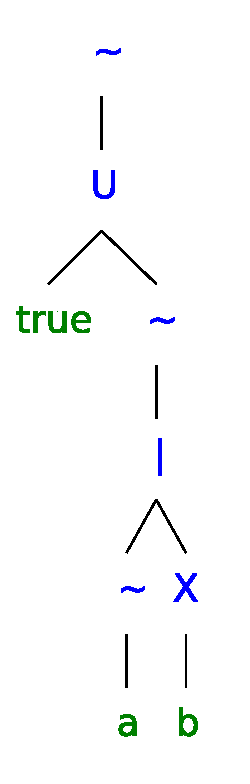
\includegraphics[height=15em, width=7.5em]{images/formula-syntax-tree}
	\caption{The syntax tree generated for the formula $"G(a \thicksim Xb)"$. Symbols are in green while operators are in blue.}
	\label{fig:formula-syntax-tree}
\end{figure}
Finally, as in the \texttt{MyLexer} class, we have to handle errors defining a specific method.

\LTLfToDFA can be used just for the parsing phase of an 	\LTLf formula as shown in Listing \ref{code:ltlf2dfa-only-parsing}.
\begin{lstlisting}[language=Python, style=Python, label={code:ltlf2dfa-only-parsing}, caption={How to use only the parsing phase of \LTLfToDFA.}]
from ltlf2dfa.Parser import MyParser

formula = "G(a->Xb)"
parser = MyParser()
parsed_formula = parser(formula)

print(parsed_formula) # syntax tree as tuple of tuples
\end{lstlisting}
\subsection{Translator.py}
The \texttt{Translator.py} module contains the majority of APIs that the \LTLfToDFA package exposes. Indeed, this module consists of a \texttt{Translator} class which concerns the core feature of the package: the translation of an \LTLf  formula into a \DFA. Since the package takes advantage of the \MONA tool for the formula conversion, the \texttt{Translator} class has to translate first the given formula into the syntax recognized by \MONA, then create the input program for \MONA and, finally, invoke \MONA to get back the resulting \DFA in the Graphviz\footnote{Graphviz is open source graph visualization software. For further details see \href{https://www.graphviz.org}{https://www.  .org}} format. 
The main methods of the \texttt{Translator} class are:
\begin{itemize}
\item \texttt{translate()}, which starting from the formula syntax tree generated (Figure \ref{fig:formula-syntax-tree}) in the parsing phase translates it into a string using the syntax of \MONA;
\item \texttt{createMonafile(flag)}, which, as the name suggests, creates the program \textit{.mona} that will be given as input to \MONA. The flag parameter is going to be \texttt{True} of \texttt{False} whether we need to compute also \declare  assumptions or not;
\item \texttt{invoke\_mona()}, which invokes \MONA in order to obtain the \DFA.
\end{itemize}
Now we will go into details of the methods stated above showing their implementation.
\subsubsection{The \texttt{translate} method}
The \texttt{translate} method is a crucial step towards reaching a good result and performance. Formally, the translation procedure from an \LTLf formula to the \MONA syntax is done passing through \FOL as shown in \ref{eq:translation-procedure}.
\begin{equation}\label{eq:translation-procedure}
\textsc{LTL}_f \rightarrow \textsc{FOL} \rightarrow \textsc{MONA}
\end{equation}
The former translation from \LTLf to \FOL is done accordingly to \citep{de2013linear}, while the latter follows from \citep{monamanual2001}.
In Listing \ref{code:ltlf2dfa-translate-method} we can see the translation's implementation. Three dots $\dots$ represent omitted code.
\begin{lstlisting}[language=Python, style=Python, escapechar = £,  label={code:ltlf2dfa-translate-method}, caption={The \texttt{translate} method.}]
import ...

class Translator:
    ...
    
    def translate(self):
        self.translated_formula = translate_bis(self.parsed_formula, \
        var='v_0')+";\n"

   ...

def translate_bis(formula_tree, var):£\label{line:translate_bis}£
    if type(formula_tree) == tuple:
        #enable this print to see the tree pruning
        # print(self.parsed_formula)
        # print(var)
        if formula_tree[0] == '&':
            # print('computed tree: '+ str(self.parsed_formula))
            if var == 'v_0':
                a = translate_bis(formula_tree[1], '0')
                # a = translate_bis(self.parsed_formula[1], '0')
                b = translate_bis(formula_tree[2], '0')
            else:
                a = translate_bis(formula_tree[1], var)
                b = translate_bis(formula_tree[2], var)
            if a == 'false' or b == 'false':
                return 'false'
            elif a == 'true':
                if b == 'true': return 'true'
            elif b == 'true': return a
            else: return '('+a+' & '+b+')'
        elif formula_tree[0] == '|':
            # print('computed tree: '+ str(self.parsed_formula))
            if var == 'v_0':
                a = translate_bis(formula_tree[1], '0')
                b = translate_bis(formula_tree[2], '0')
            else:
                a = translate_bis(formula_tree[1], var)
                b = translate_bis(formula_tree[2], var)
            if a == 'true' or b == 'true':
                return 'true'
            elif a == 'false':
                if b == 'true': return 'true'
                elif b == 'false': return 'false'
                else: return b
            elif b == 'false': return a
            else: return '('+a+' | '+b+')'
        elif formula_tree[0] == '~':
            # print('computed tree: '+ str(self.parsed_formula))
            if var == 'v_0': a = translate_bis(formula_tree[1], '0')
            else: a = translate_bis(formula_tree[1], var)
            if a == 'true': return 'false'
            elif a == 'false': return 'true'
            else: return '~('+ a +')'
        elif formula_tree[0] == 'X':
            # print('computed tree: '+ str(self.parsed_formula))
            new_var = _next(var)
            a = translate_bis(formula_tree[1],new_var)
            if var == 'v_0':
                return '('+ 'ex1 '+new_var+': '+ new_var +' = 1 '+ '& '+ \
                a +')'
            else:
                return '('+ 'ex1 '+new_var+': '+ new_var +' = '+ var + \
                ' + 1 '+ '& '+ a +')'
        elif formula_tree[0] == 'U':
            # print('computed tree: '+ str(self.parsed_formula))
            new_var = _next(var)
            new_new_var = _next(new_var)
            a = translate_bis(formula_tree[2],new_var)
            b = translate_bis(formula_tree[1],new_new_var)

            if var == 'v_0':
                if b == 'true': return '( '+ 'ex1 '+new_var+': 0 <= '+ \
                new_var+' & '+ new_var+' <= max($) & '+ a +' )'
                elif a ==  'true': return '( '+ 'ex1 '+new_var+': 0 <= '+ \
                new_var+' & '+new_var+' <= max($) & all1 '+ \
                new_new_var+': 0 <= '+new_new_var+' & '+ \
                new_new_var+' < '+new_var+' => '+b+' )'
                elif a == 'false': return 'false'
                else: return '( '+ 'ex1 '+new_var+': 0 <= '+new_var+ \
                ' & '+new_var+' <= max($) & '+ a +' & all1 '+ \
                new_new_var+': 0 <= '+new_new_var+' & '+ \
                new_new_var+' < '+new_var+' => '+b+' )'
            else:
                if b == 'true': return '( '+ 'ex1 '+new_var+': '+var+ \
                ' <= '+new_var+' & '+new_var+' <= max($) & '+ a +' )'
                elif a ==  'true': return '( '+ 'ex1 '+new_var+': '+var+ \
                ' <= '+new_var+' & '+new_var+' <= max($) & all1 '+ \ 
                new_new_var+': '+var+' <= '+new_new_var+' & '+ \ 
                new_new_var+' < '+new_var+' => '+b+' )'
                elif a == 'false': return 'false'
                else: return '( '+ 'ex1 '+new_var+': '+var+' <= '+ \ 
                new_var+' & '+new_var+' <= max($) & '+ a + \
                ' & all1 '+new_new_var+': '+var+' <= '+new_new_var+\
                ' & '+new_new_var+' < '+new_var+' => '+b+' )'
        elif formula_tree[0] == 'Y':
            # print('computed tree: '+ str(self.parsed_formula))
            new_var = _next(var)
            a = translate_bis(formula_tree[1],new_var)
            if var == 'v_0':
                return '('+ 'ex1 '+new_var+': '+ new_var + \
                ' = max($) - 1 '+ '& max($) > 0 & '+ a +')'
            else:
                return '('+ 'ex1 '+new_var+': '+ new_var + \
                ' = '+ var + ' - 1 '+ '& '+new_var+' > 0 & '+ a +')'
        elif formula_tree[0] == 'S':
            # print('computed tree: '+ str(self.parsed_formula))
            new_var = _next(var)
            new_new_var = _next(new_var)
            a = translate_bis(formula_tree[2],new_var)
            b = translate_bis(formula_tree[1],new_new_var)

            if var == 'v_0':
                if b == 'true': return '( '+ 'ex1 '+new_var+': 0 <= '+ \ 
                new_var+' & '+new_var+' <= max($) & '+ a +' )'
                elif a ==  'true': return '( '+ 'ex1 '+new_var+ \
                ': 0 <= '+new_var+' & '+new_var+ \
                ' <= max($) & all1 '+new_new_var+': '+new_var+' < '+ \ 
                new_new_var+' & '+new_new_var+' <= max($) => '+b+' )'
                elif a == 'false': return 'false'
                else: return '( '+ 'ex1 '+new_var+': 0 <= '+ \ 
                new_var+' & '+new_var+' <= max($) & '+ a + \
                ' & all1 '+new_new_var+': '+new_var+' < '+ \
                new_new_var+' & '+new_new_var+' <= max($) => '+b+' )'
            else:
                if b == 'true': return '( '+ 'ex1 '+new_var+ \ 
                ': 0 <= '+new_var+' & '+new_var+' <= max($) & '+ a +' )'
                elif a ==  'true': return '( '+ 'ex1 '+new_var+ \
                ': 0 <= '+new_var+' & '+new_var+' <= '+var+ \
                ' & all1 '+new_new_var+': '+new_var+' < '+ \
                new_new_var+' & '+new_new_var+' <= '+var+' => '+b+' )'
                elif a == 'false': return 'false'
                else: return '( '+ 'ex1 '+new_var+': 0 <= '+ \ 
                new_var+' & '+new_var+' <= '+var+' & '+ a +' & all1 '+ \ 
                new_new_var+': '+new_var+' < '+new_new_var+' & '+ \ 
                new_new_var+' <= '+var+' => '+b+' )'
    else:
        # handling non-tuple cases
        if formula_tree[0] == 'T': return 'true'
        elif formula_tree[0] == 'F': return 'false'

        # enable if you want to see recursion
        # print('computed tree: '+ str(self.parsed_formula))

        # BASE CASE OF RECURSION
        else:
            if formula_tree.isalpha():
                if var == 'v_0':
                    return '0 in '+ formula_tree.upper()
                else:
                    return var + ' in ' + formula_tree.upper()
            else:
                return var + ' in ' + formula_tree

def _next(var):
    if var == '0': return 'v_1'
    else:
        s = var.split('_')
        s[1] = str(int(s[1])+1)
        return '_'.join(s)
\end{lstlisting}
As we can see, the \texttt{translate} method is actually very simple. In fact, it just calls the \texttt{translate\_bis} function (line \ref{line:translate_bis}) to perform the proper translation. The function works in a recursive fashion taking as input the parsed formula and a variable and outputting a string containing the result. Obviously, when an instance of the \texttt{Translator} class is created the input formula is checked to have either only future or past operators.
The base case of the recursion handles the translation of symbols as they are the leaves of the syntax tree composed in the parsing phase (Figure \ref{fig:formula-syntax-tree}). On the other hand, the recursive step regards the handling of operators (non leaf components of the syntax tree) which are in our case $\lAND$, $\lOR$, $\NOT$, \Next, $\lUntil$, \Yesterday, $\Since$. During the translation, we simplify the resulting formula by avoiding pieces of the expression that are logically \texttt{True} or \texttt{False}. This simplification has two main advantages. First, it substantially reduces the length of the resulting formula, improving its readability. Second, it increases the computation performances of \MONA.
Additionally, since the \MONA syntax requires the declaration of the free variables, the \texttt{translate\_bis} function has to compute also the appriopriate free variables declaration. In this terms, the translation function uses the \texttt{\_next} function to compute the next variable each time is needed.

\subsubsection{The \texttt{createMonafile} method}
The \texttt{createMonafile} method is employed to write the program \textit{.mona} and save it in the main directory. It takes as input a boolean flag that, as stated before, stands for indicating whether one would like to compute and add the \declare assumption or not. In particular, in formal logic, as stated in \citep{DeGiacomo:2014:RLF:2893873.2894033}, the \declare assumption is expressed as in \ref{eq:declare-ass}.
\begin{equation}\label{eq:declare-ass}
\Always (\bigvee_{a \in \P} a) \lAND \Always (\bigwedge_{a,b \in \P, a \neq b} a \rightarrow \NOT b) 
\end{equation}
It consists essentially in two parts joined by the $\lAND$ operator. The former indicates that it is always true that at each point in time only one symbol is $\true$, while the latter means that always for each couple of different symbols in the formula if one is $\true$ the other must be $\false$.
The practical part can be seen in Listing \ref{code:ltlf2dfa-createmona-method}.
\begin{lstlisting}[language=Python, style=Python, escapechar = £, label={code:ltlf2dfa-createmona-method}, caption={The \texttt{createMonafile} method.}]
...
    def compute_declare_assumption(self):£\label{line:declare-ass-method}£
        pairs = list(it.combinations(self.alphabet, 2))

        if pairs:
            first_assumption = "~(ex1 y: 0<=y & y<=max($) & ~("
            for symbol in self.alphabet:
                if symbol == self.alphabet[-1]: first_assumption += \ 
                'y in '+ symbol +'))'
                else : first_assumption += 'y in '+ symbol +' | '

            second_assumption = "~(ex1 y: 0<=y & y<=max($) & ~("
            for pair in pairs:
                if pair == pairs[-1]: second_assumption += '(y notin '+ \
                pair[0]+' | y notin '+pair[1]+ ')));'
                else: second_assumption += '(y notin '+ pair[0]+ \
                ' | y notin '+pair[1]+ ') & '

            return first_assumption +' & '+ second_assumption
        else:
            return None

    def buildMonaProgram(self, flag_for_declare):£\label{line:build-mona-program}£
        if not self.alphabet and not self.translated_formula:
            raise ValueError
        else:
            if flag_for_declare:
                if self.compute_declare_assumption() is None:
                    if self.alphabet:
                        return self.headerMona + \
                        'var2 ' + ", ".join(self.alphabet) + ';\n' + \
                         self.translated_formula
                    else:
                        return self.headerMona + self.translated_formula
                else: return self.headerMona + 'var2 ' +\
                 ", ".join(self.alphabet) + ';\n' + \
                 self.translated_formula + \
                 self.compute_declare_assumption()
            else:
                if self.alphabet:
                    return self.headerMona + 'var2 ' +\
                     ", ".join(self.alphabet) + ';\n' + \
                     self.translated_formula
                else:
                    return self.headerMona + self.translated_formula

    def createMonafile(self, flag):
        program = self.buildMonaProgram(flag)
        try:
            with open('./automa.mona', 'w+') as file:
                file.write(program)
                file.close()
        except IOError:
            print('Problem with the opening of the file!')
...            
\end{lstlisting}
As shown in the code, the \texttt{createMonafile} method calls another method, the \texttt{buildMonaProgram} (line \ref{line:build-mona-program}), which literally builds the \textit{.mona} program by joining all pieces that should belong to it. Instead, regarding the \declare assumption, if needed, it is added to the \textit{.mona} program directly translated through \texttt{compute\_declare\_assumption} method at line \ref{line:declare-ass-method}.
\subsubsection{The \texttt{invoke\_mona} method}
Finally, the \texttt{invoke\_mona} method is the one that executes the \MONA compiled executable giving it the \textit{.mona} program. Consequently, the \DFA resulting from the computation of \MONA will be stored in the main directory. As stated in \ref{sec:intro}, the \LTLfToDFA package requires \MONA to be installed. Indeed, without this requirements the \texttt{invoke\_mona} method will raise an error. The implementation can be seen in Listing \ref{code:ltlf2dfa-invokemona-method}.
\begin{lstlisting}[language=Python, style=Python, escapechar = £, label={code:ltlf2dfa-invokemona-method}, caption={The \texttt{invoke\_mona} method.}]
...
    def invoke_mona(self, path='./inter-automa'):
        if sys.platform == 'linux':
            package_dir = os.path.dirname(os.path.abspath(__file__))
            mona_path = pkg_resources.resource_filename('ltlf2dfa','mona')
            if os.access(mona_path, os.X_OK):  #check if mona is executable
                try:
                    subprocess.call(package_dir+'/./mona -u -gw ' + \
                    './automa.mona > ' + path + '.dot', shell=True)
                except subprocess.CalledProcessError as e:
                    print(e)
                    exit()
                except OSError as e:
                    print(e)
                    exit()
            else:
                print('[ERROR]: MONA tool is not executable...')
                exit()
        else:
            try:
                subprocess.call('mona -u -gw ./automa.mona > ' + path + \
                '.dot', shell=True)
            except subprocess.CalledProcessError as e:
                print(e)
                exit()
            except OSError as e:
                print(e)
                exit()
...            
\end{lstlisting}
To the execute of the \MONA tool we have leveraged the built-in module \texttt{subprocess} that enables to spawn new processes, connect to their input/output/error pipes, and obtain their return codes.

Unfortunately, the \DFA resulting from \MONA needs to be post-processed because of some extra states added for other purposes not relevant for us. This aspect will be better explained in the following subsection \ref{sec:dot-handler}. 
\subsection{DotHandler.py}\label{sec:dot-handler}
The \texttt{DotHandler} class has been created in order to manage separately and better the post-processing of the \DFA, in \textit{.dot} format, resulting from the computation of \MONA. Indeed, since \MONA has been developed for different purposes, its output has an additional initial state and transition that to our intent are completely meaningless. 

Additionally, the interaction with the \textit{.dot} format has been implemented thanks to the \texttt{dotpy} library (available on GitHub\footnote{https://github.com/Francesco17/dotpy}) developed for this specific purpose paying particular attention to performances.

As we can see in the implementation of the \texttt{DotHandler} class in Listing \ref{code:ltlf2dfa-dothandler}, the main methods are \texttt{modify\_dot} and \texttt{output\_dot}.
\begin{lstlisting}[language=Python, style=Python, escapechar = £, label={code:ltlf2dfa-dothandler}, caption={The \texttt{DotHandler} class.}]
from dotpy.parser.parser import MyParser
import os

class DotHandler:

    def __init__(self, path='./inter-automa.dot'):
        self.dot_path = path
        self.new_digraph = None

    def modify_dot(self):£\label{line:modifydot}£
        if os.path.isfile(self.dot_path):
            parser = MyParser()
            with open(self.dot_path, 'r') as f:
                dot = f.read()
                f.close()

            graph = parser(dot)
            if not graph.is_singleton():
                graph.delete_node('0')
                graph.delete_edge('init', '0')
                graph.delete_edge('0', '1')
                graph.add_edge('init', '1')
            self.new_digraph = graph
        else:
            print('[ERROR] - No file DOT exists')
            exit()

    def delete_intermediate_automaton(self):
        if os.path.isfile(self.dot_path):
            os.remove(self.dot_path)
            return True
        else:
            return False

    def output_dot(self, result_path='./automa.dot'):£\label{line:outputdot}£
        try:
            if self.delete_intermediate_automaton():
                with open(result_path, 'w+') as f:
                    f.write(str(self.new_digraph))
                    f.close()
            else:
                raise IOError('[ERROR] - Something wrong occurred in '+ \
                'the elimination of intermediate automaton.')
        except IOError:
            print('[ERROR] - Problem with the opening of the file %s!' \
            %result_path)
\end{lstlisting}
The former method at line \ref{line:modifydot} takes advantage of the APIs exposed by \texttt{dotpy}. Especially, it parses the \textit{.dot} file output of \MONA (Figure \ref{fig:mona-output}), deletes the starting node $0$ and the edge from node $0$ to node $1$ and, finally, makes node $1$ initial. Consequently, the latter method at line \ref{line:outputdot} manages the output of the final post-processed \DFA (Figure \ref{fig:automa-post-processed}) and stores it in the main directory.
For instance, in Figure \ref{fig:pre-post-automaton} we can see graphically what is the outcome of the post-processing of the automaton corresponding to the formula $\varphi = \Always (a \rightarrow \Next b)$.
\begin{figure}[h]
\centering
\begin{subfigure}{.5\textwidth}
  \centering
  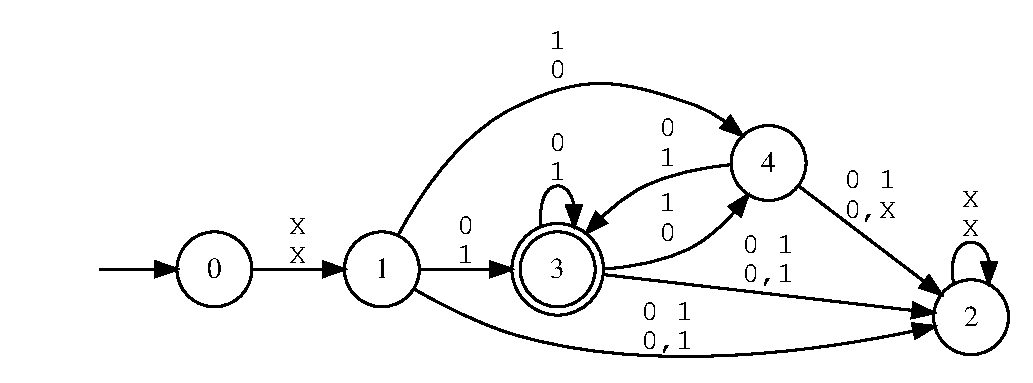
\includegraphics[width=\linewidth]{images/pre-automaton.eps}
  \caption{The \DFA output from \MONA}
  \label{fig:mona-output}
\end{subfigure}%
\begin{subfigure}{.5\textwidth}
  \centering
  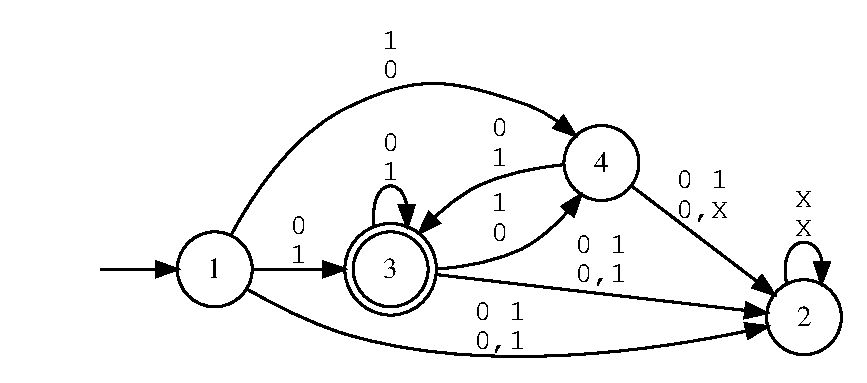
\includegraphics[width=\linewidth]{images/post-automaton.eps}
  \caption{The \DFA post-processed}
  \label{fig:automa-post-processed}
\end{subfigure}
\caption{Before and after \DFA post-processing}
\label{fig:pre-post-automaton}
\end{figure}
\section{Comparison with FLLOAT}
\section{Discussion}
In this chapter, we have presented the \LTLfToDFA Python package. We have also described the structure of the package, discussed in detail its implementation highlighting all the main features and, finally, seen how it performs with respect to time and memory relatively to the FLLOAT Python package.



















	\chapter{Planning for \LTLf/\PLTL Goals}\label{ch:planning}
In this chapter, we will define a new approach to the problem of non-deterministic planning for extended temporal goals. In particular, we will give a solution to this problem reducing it to a fully observable non-deterministic (\FOND) problem and taking advantage of our tool \LTLfToDFA, presented in Chapter \ref{ch:ltlf2dfa}. First of all, we will introduce the main idea and motivations supporting our approach. Then, we will give some preliminaries explaining the Planning Domain Definition Language (\PDDL) language and the \FOND planning problem formally. After that, we will illustrate our \FONDFOR approach with the encoding of temporal goals into a \PDDL domain and problem. Finally, we will present our practical implementation of the proposed solution.
\section{Idea and Motivations}\label{sec:plan-idea-motiv}
Planning for temporally extended goals with \textit{deterministic} actions has been well studied during the years starting from \citep{bacchus1998planning} and \citep{doherty2001talplanner}. Two main reasons why temporally extended goals have been considered over the classical goals, viewed as a desirable set of final states to be reached, are because they are not limited in what they can specify and they allows us to restrict the manner used by the plan to reach the goals. Indeed, temporal extended goals are fundamental for the specification of a collection of real-world planning problems. Yet, many of these real-world planning problems have a \textit{non-deterministic} behavior owing to unpredictable environmental conditions. However, planning for temporally extended goals with \textit{non-deterministic} actions is a more challenging problem and has been of increasingly interest only in recent years with \citep{camacho2017non, de2018automata}.

In this scenario, we have devised a solution to this problem that exploits the translation of a temporal formula to a \DFA, using \LTLfToDFA. In particular, our idea is the following: given a non-deterministic planning problem and a temporal formula, we first obtain the corresponding \DFA of the temporal formula through \LTLfToDFA, then, we encode such a \DFA into the non-deterministic planning domain. As a result, we have reduced the original problem to a classic \FOND planning problem. In other words, we compile extended temporal goals together with the original planning domain, specified in \PDDL, which is suitable for input to standard (\FOND) planners.
\section{Preliminaries}
In this section, we will give some basics on the \PDDL specification language for domains and problems of planning and a general formalization of \FOND planning.
\subsection{\PDDL}\label{sec:pddl}
As stated before, \PDDL is the acronym for Planning Domain Definition Language, which is the \textit{de-facto} standard language for representing ``classical'' planning tasks. A general planning task has the following components:
\begin{itemize}
\item Objects: elements in the world that are of our interest;
\item Predicates: objects properties that can be true or false;
\item Initial state: state of the world where we start;
\item Goal state: things we want to be true;
\item Action/Operator: rule that changes the state. 
\end{itemize}
Moreover, planning tasks are composed by two files: the \textit{domain} file where are defined predicates and actions and a \textit{problem} file where are defined objects, the initial state and the goal specification.
\subsubsection{The \textit{domain} file} 
The \textit{domain} definition gives each domain a name and specifies predicates and actions available in the domain. It might also specify types, constants and other things. A simple domain has the following format:
\begin{lstlisting}[language=PDDL, escapechar=£, label={code:pddl-domain}]
(define (domain DOMAIN_NAME)
  (:requirements [:strips] [:equality] [:typing] [:adl] ...)
  [(:types T1 T2 T3 T4 ...)]
  (:predicates (PREDICATE_1_NAME [?A1 ?A2 ... ?AN])
                (PREDICATE_2_NAME [?A1 ?A2 ... ?AN])
	       ...)

  (:action ACTION_1_NAME
    [:parameters (?P1 ?P2 ... ?PN)]
    [:precondition PRECOND_FORMULA]
    [:effect EFFECT_FORMULA]
   )
  (:action ACTION_2_NAME
    ...)
  ...)  
\end{lstlisting}
where \texttt{[]} indicates optional elements. To begin with, any \PDDL \textit{domain} definition must declare its expressivity requirements given after the \texttt{:requirements} key. The basic \PDDL expressivity is called \textsc{strips}\footnote{\textsc{strips} stands for STanford Research Institute Problem Solver, which is a formal language of inputs to the homonym automated planner developed in 1971.}, whereas a more complex one is the Action Description Language (\textsc{adl}), that extends \textsc{strips} in several ways, such as providing support for negative preconditions, disjunctive preconditions, quantifiers, conditional effects etc.. Nevertheless, many planners do not support full \textsc{adl} because creating plans efficiently is not trivial. Although the presence of this limitation, the \PDDL language allows us to use only some of the \textsc{adl} features. Furthermore, there are also other requirements often used that can be specified as \texttt{equality}, allowing the usage of the predicate \texttt{=} interpreted as equality, and \texttt{typing} allowing the typing of objects. As we will explain later in Section \ref{sec:planning-implementation}, our practical implementation supports, for now, only simple \textsc{adl}, namely conditional effects in domain's operators which do not have any nested subformula.

Secondly, there is the predicates definition after the \texttt{:predicates} key. Predicates may have zero or more parameters variables and they specify only the number of arguments that a predicate should have. Moreover, a predicate may also have typed parameters written as \texttt{?X -- TYPE\_OF\_X}.

Thirdly, there is a list of action definitions. An action is composed by the following items:
\begin{itemize}
\item \textit{parameters}: they stand for free variables and are represented with a preceding question mark \texttt{?};
\item \textit{precondition}: it tells when an action can be applied and, depending on given requirements, it could be differently defined (i.e. conjunctive formula, disjunctive formula, quantified formula, etc.);
\item \textit{effect}: it tells what changes in the state after having applied the action. As for the precondition, depending on given requirements, it could be differently defined (i.e. conjunctive formula, conditional formula, universally quantified formula, etc.)
\end{itemize}

In particular, in pure \textsc{strips} domains, the precondition formula can be one of the following:
\begin{itemize}
\item an atomic formula as \texttt{(PREDICATE\_NAME ARG1 ... ARG\_N)}
\item a conjunction of atomic formulas as \texttt{(and ATOM1 ... ATOM\_N)}
\end{itemize}
where arguments must either be parameters of the action or constants.

If the \textit{domain} uses the \texttt{:adl} or \texttt{:negated-precondition} an atomic formula could be expressed also as  \texttt{(not (PREDICATE\_NAME ARG1 ... ARG\_N))}. In addition, if the domain uses \texttt{:equality}, an atomic formula may also be of the form \texttt{(= ARG1 ARG2)}.

On the contrary, in \textsc{adl} domains, a precondition formula could be one of the following:
\begin{itemize}
\item a general negation as \texttt{(not CONDITION\_FORMULA)}
\item a conjunction of condition formulas as \texttt{(and CONDITION\_FORMULA1 ... \\CONDITION\_FORMULA\_N)}
\item a disjunction of condition formulas as \texttt{(or CONDITION\_FORMULA1 ... \\CONDITION\_FORMULA\_N)}
\item an implication as \texttt{(imply CONDITION\_FORMULA1 ... CONDITION\_FORMULA\_N)}
\item an implication as \texttt{(imply CONDITION\_FORMULA1 ... CONDITION\_FORMULA\_N)}
\item a universally quantified formula as \texttt{(forall (?V1 ?V2 ...) CONDITION\_FORMULA)}
\item an existentially quantified formula as \texttt{(exists (?V1 ?V2 ...)\\ CONDITION\_FORMULA)}
\end{itemize}

The same division can be carried out with effects formulas. Specifically, in pure \textsc{strips} domains, the precondition formula can be one of the following:
\begin{itemize}
\item an added atom as \texttt{(PREDICATE\_NAME ARG1 ... ARG\_N)}
\item a deleted atom as \texttt{(not (PREDICATE\_NAME ARG1 ... ARG\_N))}
\item a conjunction of effects as \texttt{(and ATOM1 ... ATOM\_N)}
\end{itemize}
On the other hand, in an \textsc{adl} domains, an effect formula can be expressed as:
\begin{itemize}
\item a conditional effect as \texttt{(when CONDITION\_FORMULA EFFECT\_FORMULA)}, where the \texttt{EFFECT\_FORMULA} is occur only if the \texttt{CONDITION\_FORMULA} holds true. A conditional effect can be placed within quantification formulas.
\item a universally quantified formula as \texttt{(forall (?V1 ?V2 ...) EFFECT\_FORMULA)}
\end{itemize}

As last remark that we will deepen later in Section \ref{sec:fond}, when the \PDDL \textit{domain} has \textit{non-deterministic} actions, the effect formula of those actions expresses the non-determinism with the keyword \texttt{oneof} as \texttt{(oneof (EFFECT\_FORMULA\_1) ... \\ (EFFECT\_FORMULA\_N)}.

In the following, we show a simple example of \PDDL \textit{domain}.

\begin{example}\label{ex:pddl-domain}
A simple \PDDL \textit{domain} the Tower of Hanoi game. This game consists of three rods and $n$ disks of different size, which can slide into any rods. At the beginning, disks are arranged in a neat stack in ascending order of size on a rod, the smallest on the top. The goal of the game is to move the whole stack to another rod, following three rules:
\begin{itemize}
\item one disk at a time can be moved;
\item a disk can be moved only if it is the uppermost disk on a stack;
\item no disk can be placed on top of a smaller disk.
\end{itemize}
\begin{lstlisting}[language=PDDL, escapechar=£]
(define (domain hanoi) ;comment£\label{line:domain-name}£
  (:requirements :strips :negative-preconditions :equality)£\label{line:requirements}£
  (:predicates (clear ?x) (on ?x ?y) (smaller ?x ?y) )£\label{line:predicates}£
  (:action move
    :parameters (?disc ?from ?to)£\label{line:parameters}£
    :precondition (and£\label{line:precond}£
       (smaller ?disc ?to) (smaller ?disc ?from)
       (on ?disc ?from)
       (clear ?disc) (clear ?to)
       (not (= ?from ?to))
    )
    :effect (and£\label{line:effects}£
      (clear ?from)
      (on ?disc ?to)
      (not (on ?disc ?from))
      (not (clear ?to))
    )
  )
)
\end{lstlisting}
The \PDDL \textit{domain} file of the Tower of Hanoi is quite simple. Indeed, it consists of only one action (\texttt{move}) and only a few predicates. Firstly, the name given to this \textit{domain} is \texttt{hanoi}. Then, there have been specified requirements as \texttt{:strips}, \texttt{:negative-preconditions} and \texttt{:equality}. After that, at line \ref{line:predicates}, there is the definition of all predicates involved in the \PDDL \textit{domain}. In particular, there are three predicates to describe if the top of a disk is \texttt{clear}, which disk is \texttt{on} top of another and, finally, which disk is \texttt{smaller} than another. Finally, there is the \texttt{move} action declaration with its parameters, its precondition formula and its effect formula.
\end{example}
\subsubsection{The \textit{problem} file} 
After having examined how a \PDDL \textit{domain} is defined, we can see the formulation of a \PDDL \textit{problem}. A \PDDL \textit{problem} is what a planner tries to solve. The \textit{problem} file has the following format:
\begin{lstlisting}[language=PDDL, escapechar=£, label={code:pddl-domain}]
(define (problem PROBLEM_NAME)
  (:domain DOMAIN_NAME)
  (:objects OBJ1 OBJ2 ... OBJ_N)
  (:init ATOM1 ATOM2 ... ATOM_N)
  (:goal CONDITION_FORMULA)
  )
\end{lstlisting}
At a first glance, we can notice that the \textit{problem} definition includes the specification of the domain to which it is related. Indeed, every problem is defined with respect to a precise \textit{domain}. Then, there is the object list which could be typed or untyped. After that, there are the initial and goal specification, respectively. The former defines what is true at the beginning of the planning task and it consists of ground atoms, namely predicates instantiated with previously defined objects. Finally, the goal description represents the formula, consisting of instantiated predicates, that we would like to achieve and obtain as a final state.
In the following, we show a simple example of \PDDL \textit{problem}.

\begin{example}
In this example, we show a possible \PDDL \textit{problem} for the Tower of Hanoi game for which we have shown the \textit{domain} in the Example \ref{ex:pddl-domain}.
\begin{lstlisting}[language=PDDL, escapechar=£]
(define (problem hanoi-prob)
  (:domain hanoi)
  (:objects rod1 rod2 rod3 d1 d2 d3)£\label{line:objs-prob}£
  (:init 
     (smaller d1 rod1) (smaller d2 rod1) (smaller d3 rod1)
     (smaller d1 rod2) (smaller d2 rod2) (smaller d3 rod2)
     (smaller d1 rod3) (smaller d2 rod3) (smaller d3 rod3)
     (smaller d2 d1) (smaller d3 d1) (smaller d3 d2)
     (clear rod2) (clear rod3) (clear d1)
     (on d3 rod1) (on d2 d3) (on d1 d2))
  (:goal (and (on d3 rod3) (on d2 d3) (on d1 d2)))
)
\end{lstlisting}
At line \ref{line:objs-prob}, we have three rods and three disks. At the beginning, all instantiated predicates that are true are mentioned. If a predicate is not mentioned, it is considered to be false. In the initial situation there have been specified all possible movements with the \texttt{smaller} predicate, the disks are one on top of the other in ascending order on \texttt{rod1} whereas the other two rods are \texttt{clear}. In addition, the goal description is a conjuctive formula requiring disks on a stack on the \texttt{rod3}.
\end{example}

Once both \PDDL \textit{domain} and a \textit{problem} are specified, they are given as input to planners.
\subsection{Fully Observable Non Deterministic Planning}\label{sec:fond}
In this Section, we formally define what Fully Observable Non Deterministic Planning is giving some notions and definitions. Initially, we recall some concepts of ``classical'' planning while assuming the reader to be acquainted with basics of planning.

Given a \PDDL specification with a \textit{domain} and its corresponding \textit{problem}, we would like to solve this specification in order to find a sequence of actions such that the goal formula holds true at the end of the execution. A \textit{plan} is exactly that sequence of actions which leads the agent to achieve the goal starting from the initial state. Formally, we give the following definition.

\begin{definition}\label{def:classic-planning}
A planning problem is defined as a tuple $\P = \tup{\Sigma, s_0, g}$, where:
\begin{itemize}
\item $\Sigma$ is the state-transition system;
\item $s_0$ is the initial state;
\item $g$ is the goal state.
\end{itemize}
\end{definition}

\noindent Given the above Definition \ref{def:classic-planning}, we can formally define what a plan is.

\begin{definition}\label{def:plan}
A \textit{plan} is any sequence of actions $\sigma = \tup{a_1,a_2,\dots, a_n}$ such that each $a_i$ is a ground instance of an operator defined in the domain description.
\end{definition}

\noindent Moreover, we have that:

\begin{definition}\label{def:plan-sol}
A \textit{plan} is a solution for $\P = \tup{\Sigma, s_0, g}$, if it is executable and achieves $g$.
\end{definition}

Furthermore, a ``classical'' planning problem, just defined, is given under the assumptions of \textit{fully observability} and \textit{determinism}. In particular, the former means that the agent can always see the entire state of the environment whereas the latter means that the execution of an action is certain, namely any action that the agent takes uniquely determines its outcome.

Unlike the ``classical'' planning approach, in this thesis we focus on \textit{Fully Observable Non Deterministic} (\FOND) planning. Indeed, we continue relying on the \textit{fully observability}, but loosing the \textit{determinism}. In other words, in \FOND planning we have the uncertainty on the outcome of an action execution. As anticipated in Section \ref{sec:pddl}, the uncertainty of the outcome of an operator execution is syntactically expressed, in \PDDL, with the keyword \texttt{oneof}. To better capture this concept, we give the following example.

\begin{example}
Here, we show as example the \texttt{put-on-block} operator of the \FOND version of the well-known blocksworld \PDDL \textit{domain}.
\begin{lstlisting}[language=PDDL, escapechar=£]
(:action put-on-block
  :parameters (?b1 ?b2 - block)
  :precondition (and (holding ?b1) (clear ?b2))
  :effect (oneof (and (on ?b1 ?b2) (emptyhand) (clear ?b1) £\label{line:oneof}£
                 (not (holding ?b1)) (not (clear ?b2)))
                 (and (on-table ?b1) (emptyhand) (clear ?b1) 
                 (not (holding ?b1)))
          )
)
\end{lstlisting}
The effect of the \texttt{put-on-block} is non deterministic. Specifically, the action is executed every time the agent is holding a block and another block is clear on the top. The effect can be either that the block is put on top of the other block or that the block is put on table. This has to be intended as an aleatory event. Indeed, the agent does not control the operator execution result.
\end{example}

Additionally, a \textit{non-deterministic} action $a$ with effect $oneof(E_1,\dots,E_n)$ can be intended as a set of \textit{deterministic} actions $b_1,\dots,b_n$, sharing the same precondition of $a$, but with effects $E_1,\dots,E_n$, respectively. Hence, the application of action $a$ turns out in the application of one of the actions $b_i$, chosen non-deterministically.

At this point, we can formally define the \FOND planning. Following \citep{ghallab2004automated} and \citep{geffner2013concise}, we give the following definition:
\begin{definition}
A \textit{non-deterministic domain} is a tuple $\D = \tup{2^\F, \mathcal{A}, s_0, \delta, \alpha}$ where:
\begin{itemize}
\item $\F$ is a set of \textit{fluents} (atomic propositions);
\item $\mathcal{A}$ is a set of \textit{actions} (atomic symbols);
\item $2^\F$ is the set of states;
\item $s_0$ is the initial state (initial assignment to fluents);
\item $\alpha(s) \subseteq \mathcal{A}$ represents \textit{action preconditions};
\item $(s, a, s') \in \delta$ with $a \in \alpha(s)$ represents \textit{action effects} (including frame assumptions).
\end{itemize}
\end{definition}
\noindent Such domain $\D$ is assumed to be represented compactly (e.g. in \PDDL), therefore, considering the \textit{size} of the domain as the cardinality of $\F$. Intuitively, the evolution of a non-deterministic domain is as follows: from a given state $s$, the agent chooses what action $a \in \alpha(s)$ to execute, then, the environment chooses a \textit{successor state} $s'$ with $(s,a,s') \in \delta$. To this extent, planning can also be seen as a \textit{game} between two players: the agent tries to force eventually reaching the goal no matter how the environment behaves.
Moreover, the agent can execute an action having the knowledge of all history of states so far.

Now, we can define the meaning of solving a \FOND planning problem on $\D$. A \textit{trace} of $\D$ is a finite or infinite sequence $s_0,a_0,s_1,a_1, \dots$ where $s_0$ is the initial state, $a_i \in \alpha(s_i)$ and $s_{i+1} \in \delta(s_i,a_i)$ for each $s_i,a_i$ in the trace.

Solutions to a \FOND problem $\P$ are called \textit{strategies} (or \textit{policies}). A \textit{strategy} $\trace$ is defined as follows:
\begin{definition}\label{def:policy}
Given a \FOND problem $\P$, a \textit{strategy} $\trace$ for $\P$ is a partial function defined as:
\begin{equation}
\trace: (2^\F)^+ \rightarrow \mathcal{A}
\end{equation}
such that for every $u \in (2^\F)^+$, if $\trace(u)$ is defined, then $\trace(u) \in \alpha(last(u))$, namely it selects applicable actions, whereas, if $\trace(u)$ is undefined, then $\trace(u) = \bot$.
\end{definition}
\noindent A trace $\tau$ is \textit{generated} by $\trace$ (often called $\trace$-trace) if the following holds:
\begin{itemize}
\item if $s_0,a_0,\dots,s_i,a_i$ is a prefix of $\tau$, then $\trace(s_0,s_1,\dots,s_i) = a_i$;
\item if $\tau$ is finite, i.e. $\tau = s_0,a_0,\dots,a_{n-1},s_n$, then $\trace(s_0,s_1,\dots,s_i) = \bot$.
\end{itemize}

For \FOND planning problems, in \citep{cimatti2003weak}, are defined different classes of solutions. Here we examine only two of them, namely \textit{strong solution} and \textit{strong cyclic solutions}. In the following, we give their formal definitions.

\begin{definition}\label{def:strong-sol}
A \textit{strong solution} is a strategy that is guaranteed to achieve the goal regardless of non-determinism.
\end{definition}

\begin{definition}\label{def:strong-cyc-sol}
\textit{Strong cyclic solutions} guarantee goal reachability only under the assumption of \textit{fairness}. In the presence of \textit{fairness} it is supposed that all action outcomes, in a given state, would occur infinitely often. 
\end{definition}
Obviously, \textit{strong cyclic solutions} are less restrictive than a \textit{strong solution}.
Indeed, as the name suggests, a strong cyclic solution may revisit states. However, in this thesis we will focus only on searching \textit{strong solutions}. As final remark, when searching for a strong solution to a \FOND problem we refer to \FONDS.

In the next Section, we will generalize the concept of solving \FOND planning problems with extended temporal goals, describing the step by step encoding process of those temporal goals in the \FOND domain, written in \PDDL.
\section{The \FONDFOR approach}\label{sec:fond-plan-appr}
As written in Section \ref{sec:plan-idea-motiv}, planning with extended temporal goals has been considered over the representation of goals in classical planning to capture a richer class of plans where restrictions on the whole sequence of states must be satisfied as well. In particular, differently from classical planning, where the goal description can only be expressed as a propositional formula, in planning for extended temporal goals the goal description may have the same expressive power of the temporal logic in which the goal is specified. This enlarges the general view about planning. In other words, extended temporal goals specify desirable sequences of states and a plan exists if its execution yields one of these desirable sequences \citep{bacchus1998planning}.

In this thesis, we propose a new approach, called \FONDFOR, that uses \LTLf and \PLTL formalisms as temporal logics for expressing extended goals.
To better understand the powerful of planning with extended temporal goals we give the following example.

\begin{example}\label{ex:pla-temp-simple}
Considering the well known \texttt{tireworld} \FOND planning task, one of the possible classical goal can be
*** PUT THE EXAMPLE HERE ***
\end{example}

Planning for \LTLf and \PLTL goals slightly changes the definitions given in Section \ref{sec:fond}. In the following, we give the modified definitions of the concepts seen before.

\begin{definition}\label{def:strong-sol-extend}
Given a domain $\D$ and an \LTLf/\PLTL formula $\varphi$ over atoms $\F \cup \mathcal{A}$, a strategy $\trace$ is a \textit{strong solution} to $\D$ for goal $\varphi$, if every $\trace$-trace is finite and satisfies $\varphi$.
\end{definition}

About complexity of \FONDS, we have the following Theorem.

\begin{theorem}\citep{rintanen2004complexity}
\label{th:fond-complex}
Solving \FONDS problems for \LTLf/\PLTL goals of the form $\Diamond G$ is \EXPTIME-complete in the size of the domain and \TWOEXPTIME-complete in the size of the goal.
\end{theorem}

\subsection{Idea}
Our \FONDFOR approach works as follows: given a non-deterministic planning domain $\D$, an initial state $s_0$ and an \LTLf or \PLTL goal formula $\varphi$ (whose symbols are ground predicates), we first obtain the corresponding \DFA of the temporal formula through \LTLfToDFA, then, we encode such a \DFA into the non-deterministic planning domain $\D$. As a result, we will have a new domain $\D'$ and a new problem $P'$ that can be considered and solved as a classical \FOND planning problem. 

The new approach, carried out in this thesis, stems from the research in \cite{de2018automata}, that, basically, proposes automata-theoretic foundations of \FOND planning for \LTLf goals. In particular, they compute the cartesian product between the \DFA corresponding to the domain $\D$ ($\automaton_\D$) and the \DFA corresponding to $\varphi$ ($\automaton_\varphi$), thus, solving a \DFA game on $\automaton_\D \times \automaton_\varphi$, i.e. find, if exists, a trace accepted by $\automaton_\D \times \automaton_\varphi$. Moreover, an important consideration is that the resulting automaton $\automaton_\D \times \automaton_\varphi$ will read both the action and its effect, as shown, for instance, in Figure \ref{fig:dfa-game}.

However, unlike what has been done in \cite{de2018automata}, we split transitions containing the action and its effect in order to have them separately. The reason for this separation is that having both the action and its effect on the same transition is not suitable on a practical perspective. Hence, we have devised a solution in which we run $\automaton_\D$ and $\automaton_\varphi$ separately, but combining them into a single unique transition system. To achieve this, we move $\automaton_\D$ and $\automaton_\varphi$ alternatively by introducing an additional predicate, which we will call \texttt{turnDomain}, that is true when we should move $\automaton_\D$ and is false when we should move $\automaton_\varphi$. In the following, we give an example to better understand the solution put in place in this thesis.

\begin{example}\label{ex:yale-scenario}
Let us consider the simplified version of the classical Yale shooting domain \citep{hanks1986default} as in \cite{de2018automata}, where we have that the turkey is either alive or not and the actions are shoot and wait with the obvious effects, but with a gun that can be faulty. Specifically, shooting with a (supposedly) working gun can either end in killing the turkey or in the turkey staying alive and the discovery that the gun is not working properly. On the other hand, shooting (with care) with a gun that does not work properly makes it work and kills the turkey. The cartesian product $\automaton_\D \times \automaton_\varphi$ with $\varphi = \Diamond\lnot a$ is as follows:

\begin{figure}[h]
\centering
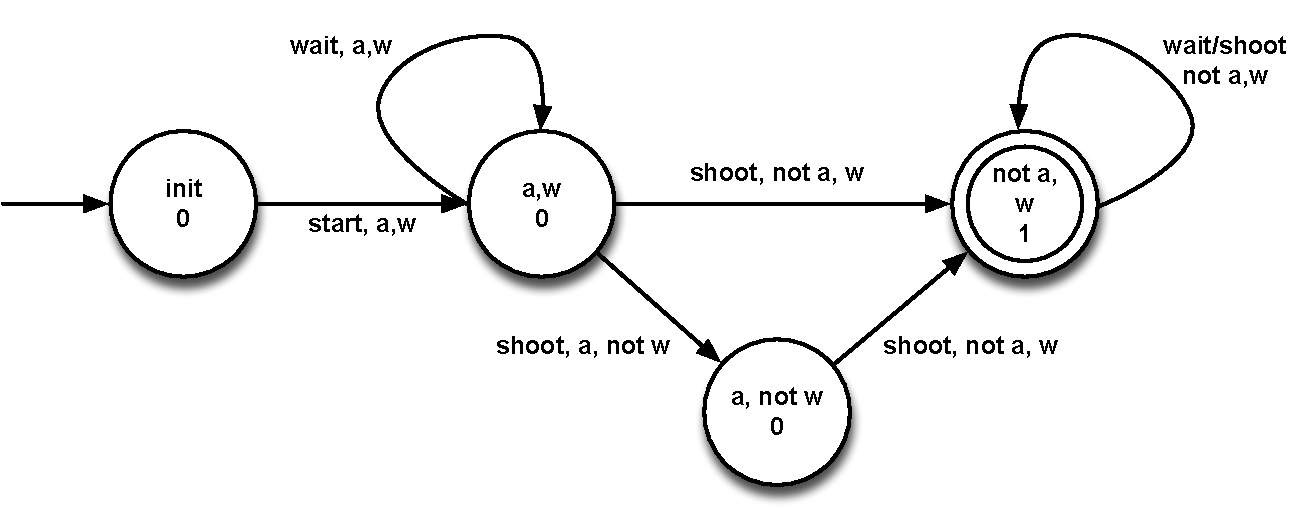
\includegraphics[width=0.7\textwidth]{images/cartesian-prod}
\caption{The \DFA corresponding to $\automaton_\D \times \automaton_\varphi$. Symbol \texttt{a} stands for \textit{alive} and \texttt{w} for \textit{working}} 
\label{fig:dfa-game}
\end{figure}

\noindent As we can see in Figure \ref{fig:dfa-game}, each transition reads both the action and its effect. This is not suitable for a practical implementation. Thus, we do not perform the cartesian product between the two automata. On the contrast, we build a transition system as follows:

\begin{figure}[h]
\centering
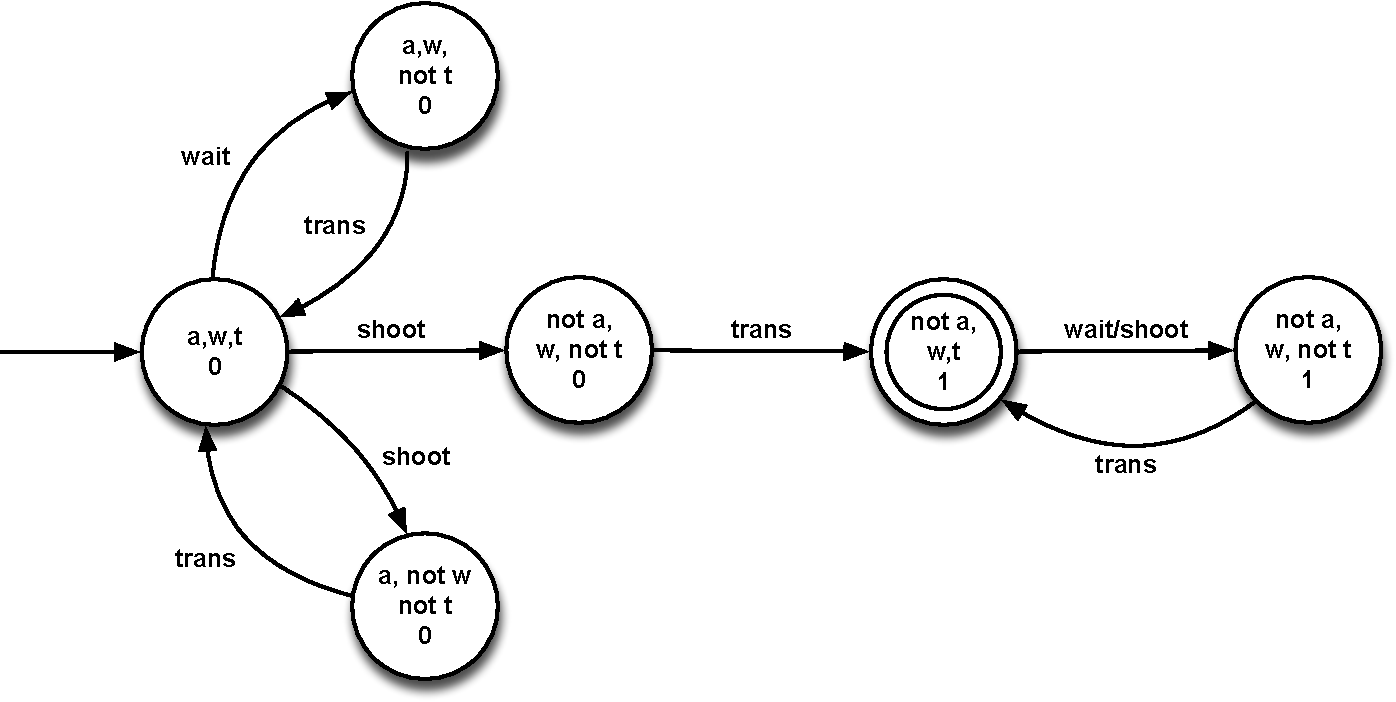
\includegraphics[width=0.8\textwidth]{images/yale-our-sol}
\caption{The new transition system corresponding to the Yale shooting domain. Symbol \texttt{a} stands for \textit{alive}, \texttt{w} for \textit{working} and \texttt{t} for \textit{turnDomain}} 
\label{fig:yale-our-sol}
\end{figure}
\end{example}

The transition system, shown in Figure \ref{fig:yale-our-sol}, expresses the new domain $\D'$ that has a perfect alternation of transitions. In particular, actions of the initial domain $\D$ alternates with a special action, that we called \texttt{trans}, representing the movement done by $\automaton_\varphi$. Moreover, it is important to notice the usage of the added predicate \texttt{turnDomain} allowing us to alternate between general actions and the new action \texttt{trans}.

In the next Section, we will explain how the new domain $\D'$ and the new problem $\P'$ can be written in \PDDL by showing the encoding of \LTLf/\PLTL goals in \PDDL.

\subsection{Encoding of \LTLf/\PLTL goals in \PDDL}
In this Section, we describe the process of obtaining the new domain $\D'$ and the new problem $\P'$, both specified in \PDDL. The original \PDDL domain $\D$ and the associated original problem $\P$ change when introducing \LTLf/\PLTL goals. In particular, what changes is the way we encode our \LTLf/\PLTL formula in \PDDL. Firstly, we employ our \LTLfToDFA tool to convert the given goal formula $\varphi$ into the corresponding \DFA. Then, we encode, in a specific way, the resulting \DFA automaton in \PDDL modifying the original domain $\D$ and problem $\P$.

\subsubsection*{Modification of Domain $\D$}
Regarding $\D$, we add the \texttt{trans} operator and some predicates depending on the resulting \DFA. Specifically, since the goal formula $\varphi$ has instantiated predicates as symbols, to capture the general representation of $\varphi$ we should consider them as variables. Hence, the formula $\varphi$ becomes $\varphi(x_1,x_2,\dots,x_n)$, where $n$ is the number of variables. As a result, the representation of the \DFA, associated to $\varphi(x_1,x_2,\dots,x_n)$, is parametric, namely both states and actions depend on variables as for the automaton in Figure \ref{fig:dfa-parametric}.

\begin{example}\label{ex:param-formula}
Let us consider the goal formula $\varphi = \Diamond(on(d3,rod3))$ for the Tower of Hanoi planning problem. The predicate \texttt{on} is instantiated on objects \texttt{d3} and \texttt{rod3}. By considering them as variables, $\varphi$ becomes $\varphi(x_1,x_2) = \Diamond(on(x_1,x_2))$, where we know that $x_1$ will correspond to $d3$ and $x_2$ to $rod3$. 
\begin{figure}[h]
\centering
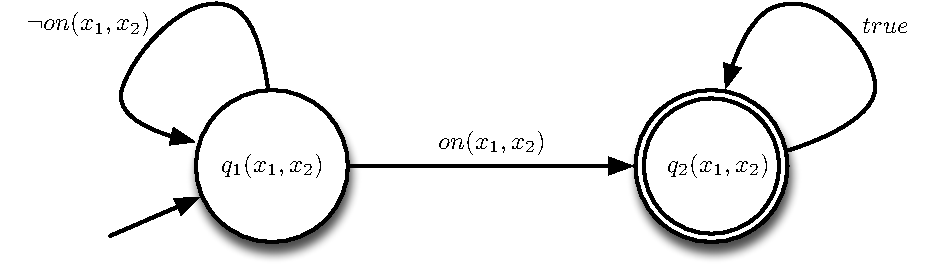
\includegraphics[width=0.7\textwidth]{images/automa-param}
\caption{The parametric \DFA corresponding to $\varphi(x_1,x_2) = \Diamond(on(x_1,x_2))$} 
\label{fig:dfa-parametric}
\end{figure}
\end{example}

At this point, we can explain how we build the new operator \texttt{trans}. Since this operator has been introduced to simulate moves of the automaton related to the goal formula, the operator will have:
\begin{itemize}
\item variables as parameters;
\item the negation of the \texttt{turnDomain} predicate as precondition;
\item transitions encoded as conditional effects as effect.
\end{itemize}
We give the following example:

\begin{example}\label{ex:trans-op-adl}
Consider the \DFA in Figure \ref{fig:dfa-parametric}, the \texttt{trans} operator built from that automaton is the following:
\begin{lstlisting}[language=PDDL, escapechar=£]
(:action trans
  :parameters (?x1 ?x2)
  :precondition (not (turnDomain))
  :effect (and (when (and (q1 ?x1 ?x2) (not (on ?x1 ?x2)))
              (and (q1 ?x1 ?x2) (not (q2 ?x1 ?x2)) (turnDomain))
          (when (or (and (q1 ?x1 ?x2) (on ?x1 ?x2)) (q2 ?x1 ?x2))£\label{line:cond-eff-ex}£
              (and (q2 ?x1 ?x2) (not (q1 ?x1 ?x2)) (turnDomain))
  )
)
\end{lstlisting}
\end{example}

As shown in Example \ref{ex:trans-op-adl}, transitions, with source state and destination state, are encoded as conditional effects, where the condition formula includes source state and formula symbols whereas the effect formula includes the destination state, the negation of all other states and \texttt{turnDomain}. Moreover, in order to get a compact encoding of \texttt{trans} effects, conditional effects are brought together by destination state as happens, for instance, at line \ref{line:cond-eff-ex}.

After the \texttt{trans} operator has been built, we change $\D$ as follows:
\begin{enumerate}
\item add \texttt{turnDomain} to all actions precondition and negated \texttt{turnDomain} to all actions effects;
\item add \texttt{trans} operator;
\item add all automaton state predicates to the domain predicates definition.
\end{enumerate}

\noindent We have thus obtained the new domain $\D'$. In the following, we show an example.

\begin{example}\label{ex:new-dom}
Let consider the Triangle Tireworld scenario. The objective is to drive from one location to another, however while driving a tire may be going flat. If there is a spare tire in the location of the car, then the car can use it to fix the flat tire. The original \PDDL domain is:
\begin{lstlisting}[language=PDDL, escapechar=£]
(define (domain triangle-tire)
  (:requirements :typing :strips :non-deterministic)
  (:types location)
  (:predicates (vehicle-at ?loc - location)
	       (spare-in ?loc - location)
	       (road ?from - location ?to - location)
	       (not-flattire))
  (:action move-car
    :parameters (?from - location ?to - location)
    :precondition (and (vehicle-at ?from) (road ?from ?to) 
      (not-flattire))
    :effect (oneof (and (vehicle-at ?to) (not (vehicle-at ?from)))
	  (and (vehicle-at ?to) (not (vehicle-at ?from)) 
	  (not (not-flattire))))
   )
  (:action changetire
    :parameters (?loc - location)
    :precondition (and (spare-in ?loc) (vehicle-at ?loc))
    :effect (and (not (spare-in ?loc)) (not-flattire))
   )
)
\end{lstlisting}
Now, consider a simple \LTLf formula $\varphi = \Diamond vehicleAt(l13)$. It requires that eventually the vehicle will be in location $l13$. The parametric \DFA associated to $\varphi(x)$ is depicted in Figure \ref{fig:dfa-parametric2}.
\begin{figure}[h]
\centering
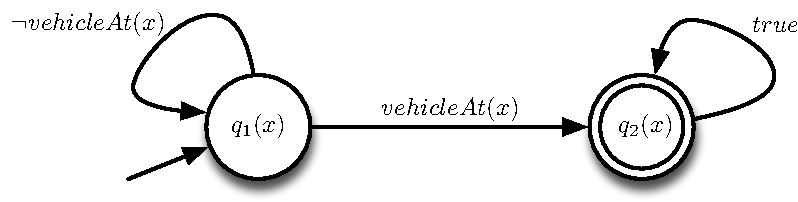
\includegraphics[width=0.7\textwidth]{images/automa-param2}
\caption{The parametric \DFA corresponding to $\varphi(x) = \Diamond(vehicleAt(x))$} 
\label{fig:dfa-parametric2}
\end{figure}

Considering the \DFA in Figure \ref{fig:dfa-parametric2}, the \texttt{trans} operator built from that automaton is the following:
\begin{lstlisting}[language=PDDL, escapechar=£]
(:action trans
  :parameters (?x - location)
  :precondition (not (turnDomain))
  :effect (and (when (and (q1 ?x) (not (vehicle-at ?x)))
              (and (q1 ?x) (not (q2 ?x)) (turnDomain))
          (when (or (and (q1 ?x) (vehicle-at ?x)) (q2 ?x))
              (and (q2 ?x) (not (q1 ?x)) (turnDomain))
  )
)
\end{lstlisting}

Finally, putting together all pieces and carrying out changes described above, we obtain the new domain $\D'$ as follows:

\begin{lstlisting}[language=PDDL, escapechar=£]
(define (domain triangle-tire)
  (:requirements :typing :strips :non-deterministic)
  (:types location)
  (:predicates (vehicle-at ?loc - location)
	       (spare-in ?loc - location)
	       (road ?from - location ?to - location)
	       (not-flattire)
	       (q1 ?x - location)
	       (q2 ?x - location)
	       (turnDomain))
  (:action move-car
    :parameters (?from - location ?to - location)
    :precondition (and (vehicle-at ?from) (road ?from ?to) 
      (not-flattire) (turnDomain))
    :effect (oneof (and (vehicle-at ?to) (not (vehicle-at ?from))
      (not (turnDomain)))
	  (and (vehicle-at ?to) (not (vehicle-at ?from)) 
	  (not (not-flattire)) (not (turnDomain))))
   )
  (:action changetire
    :parameters (?loc - location)
    :precondition (and (spare-in ?loc) (vehicle-at ?loc) 
      (turnDomain))
    :effect (and (not (spare-in ?loc)) (not-flattire)
      (not (turnDomain)))
   )
  (:action trans
    :parameters (?x - location)
    :precondition (not (turnDomain))
    :effect (and (when (and (q1 ?x) (not (vehicle-at ?x)))
              (and (q1 ?x) (not (q2 ?x)) (turnDomain))
          (when (or (and (q1 ?x) (vehicle-at ?x)) (q2 ?x))
              (and (q2 ?x) (not (q1 ?x)) (turnDomain)))
  )   
)
\end{lstlisting}
\end{example}

\subsubsection*{Modification of Problem $\P$}
Concerning the planning problem $\P$, we completely discard the goal specification, whereas the initial state description is slightly modified. Moreover, the problem name, the associated domain name and all defined objects remain unchanged. We have to modify both the initial state and the goal state specifications to make them compliant with $\D'$, containing all changes introduced in the planning domain $\D$. To this extent, in the initial state description, we should add to the original specification the new predicate \texttt{turnDomain}, meaning that it is $true$ at the beginning, and the initial state of the automaton instantiated on the objects of interest, i.e. those specified in the \LTLf/\PLTL formula $\varphi$. 

On the other hand, the goal description is built from scratch by putting together the \texttt{turnDomain} predicate, meaning that it must be $true$ at the end of the execution, and the final state(s) of the automaton always instantiated on the objects of interest. Here, it is important to notice that if the automaton has two or more final states, they should be put in disjunction.

We can give the following example.

\begin{example}\label{ex:new-prob}
Let consider again the Triangle Tireworld scenario, shown in the Example \ref{ex:new-dom}. The original \PDDL domain is:
\begin{lstlisting}[language=PDDL, escapechar=£]
(define (problem triangle-tire-1)
  (:domain triangle-tire)
  (:objects l11 l12 l13 l21 l22 l23 l31 l32 l33 - location)
  (:init (vehicle-at l11)
    (road l11 l12) (road l12 l13) (road l11 l21) (road l12 l22)
    (road l21 l12) (road l22 l13) (road l21 l31) (road l31 l22)
    (spare-in l21) (spare-in l22) (spare-in l31)
    (not-flattire))
  (:goal (vehicle-at l13))
)
\end{lstlisting}
Now, considering the same \LTLf formula $\varphi = \Diamond vehicleAt(l13)$, the object of interest is $l13$. Hence, we should evaluate our automaton states as $q_1(l13)$ and $q_2(l13)$.

Finally, putting together all pieces and carrying out changes described above, we obtain the new problem $\P'$ as follows:

\begin{lstlisting}[language=PDDL, escapechar=£]
(define (problem triangle-tire-1)
  (:domain triangle-tire)
  (:objects l11 l12 l13 l21 l22 l23 l31 l32 l33 - location)
  (:init (vehicle-at l11)
    (road l11 l12) (road l12 l13) (road l11 l21) (road l12 l22)
    (road l21 l12) (road l22 l13) (road l21 l31) (road l31 l22)
    (spare-in l21) (spare-in l22) (spare-in l31)
    (not-flattire) (turnDomain) (q1 l13))
  (:goal (and (turnDomain) (q2 l13)))
)
\end{lstlisting}
As a remark, we will refer to the new goal specification as $\G'$.
\end{example}

Having examined the encoding of \LTLf/\PLTL goal formulas in \PDDL, the resulting planning domain $\D'$ and problem $\P'$ represent a ``classical'' planning specification. In the next Section, we will see how we obtain a strong policy giving $\D'$ and $\P'$.

\subsection{\FOND Planners}
In this Section, we talk about the state-of-art \FOND planners and how they are employed within this thesis.

To begin with, thanks to our encoding process, we have reduced the problem of \FOND planning for \LTLf/\PLTL goals to a ``classical'' \FOND planning, which is essentially a \textit{reachability} problem. We can state the following Theorem.

\begin{theorem}
A strong policy $\trace$ is a valid policy for $\D', \G'$ if and only if $\trace$ is a valid policy for $\D,\varphi$.
\end{theorem}

Given this Theorem, we can solve our original problem giving $\D'$ and $\P'$ as input to standard \FOND planners. The main state-of-art \FOND planners are:
\begin{itemize}
\item MBP and Gamer, which are OBDD\footnote{OBDD stands for \textit{Ordered Binary Decision Diagram}}-based planners \citep{cimatti2003weak, kissmann2009solving}
\item MyND and Grendel, which rely on explicit AND/OR graph search \citep{bercher2010pattern, ramirez2014directed}
\item PRP, NDP and FIP, which rely on classical algorithms \citep{kuter2008using, fu2011simple, muise2012improved}
\item FOND-SAT, which provides a SAT approach to \FOND planning \citep{geffner2018compact}
\end{itemize}
Although \FOND planning is receiving an increasingly interest, the research on computational approaches has been recently reduced. Nevertheless, some planners performs well on different contexts of use. In our thesis, we are going to employ a customized version of FOND-SAT, the newest planner.

Secondly, although the description of many real-world planning problems involves the use of conditional effects, requiring full support of ADL by planners, those state-of-art planners, cited above, are still not able to fully handle such conditional effects. This represents a big limitation that can be surely deepened as a future work of this thesis. To this extent, we should first compile away conditional effects from the domain and, then, we can give it to a planner. Our proposal implementation, thoroughly described in the Section \ref{sec:planning-implementation}, is able to compile away simple conditional effects, namely those conditional effects that do not have nested formulas. Additionally, we have to  compile away conditional effects of the \texttt{trans} operator upstream even though its  representation with the employment of conditional effects is much more effective and compact. Luckily, this process consists of just splitting the operator in as many operators as the number of conditional effects present in the original action and adding the condition formula in the preconditions for each conditional effect. In the following, we make a clarifying example.

\begin{example}
The \texttt{trans} operator built in the Example \ref{ex:new-dom} is:
\begin{lstlisting}[language=PDDL, escapechar=£]
(:action trans
  :parameters (?x - location)
  :precondition (not (turnDomain))
  :effect (and (when (and (q1 ?x) (not (vehicle-at ?x)))
              (and (q1 ?x) (not (q2 ?x)) (turnDomain))
          (when (or (and (q1 ?x) (vehicle-at ?x)) (q2 ?x))
              (and (q2 ?x) (not (q1 ?x)) (turnDomain))
  )
)
\end{lstlisting}
As we can see, it contains only two conditional effects. Hence, we split this operator in two operators that we are going to call \texttt{trans-0} and \texttt{trans-1}, respectively. In particular, for each conditional effect the condition formula is added to the precondition and the effect formula is left in the effects. \texttt{trans-0} and \texttt{trans-1} are as follows:
\begin{lstlisting}[language=PDDL, escapechar=£]
(:action trans-0
  :parameters (?x - location)
  :precondition (and (and (q1 ?x) (not (vehicle-at ?x))) 
    (not (turnDomain)))
  :effect (and (q1 ?x) (not (q2 ?x)) (turnDomain))
  )
)
(:action trans-1
  :parameters (?x - location)
  :precondition (and (or (and (q1 ?x) (vehicle-at ?x)) (q2 ?x)) 
    (not (turnDomain)))
  :effect (and (q2 ?x) (not (q1 ?x)) (turnDomain))
  )
)
\end{lstlisting}
\end{example}

At this point, having compiled away simple conditional effects from the modified domain $\D'$, we can finally describe how we have employed FOND-SAT in our thesis.

The main reasons why we have chosen FOND-SAT are the following:
\begin{itemize}
\item it is written in pure Python, hence we can easily integrate it in our Python implementation as we will see in Section \ref{sec:planning-implementation};
\item it performs reasonably well;
\item it outputs all policies building a transition system whose states are called \textit{controller states}.
\end{itemize}
FOND-SAT takes also advantage of the parser and translation PDDL-to-SAS+ scripts from  PRP. When FOND-SAT was developed, PRP's translation scripts could not handle disjunctive preconditions that may be present in our \texttt{trans} operators. As a result, we have modified FOND-SAT with the newest version of those scripts directly from PRP.

The usage of FOND-SAT is really simple. From its source folder, it is necessary to run the following command in the terminal:
\begin{lstlisting}[language=bash]
python main.py -strong 1 -policy 1 /path-to/domain.pddl 
/path-to/problem.pddl
\end{lstlisting}
The command simply executes the main module of FOND-SAT requiring to find strong policies and to print, if exists, the policy found. We feed FOND-SAT with our new domain $\D'$ and new problem $\P'$.

Once strong plans are found, FOND-SAT displays the policy in four sections as follows:
\begin{itemize}
\item Atom (CS): for each controller state it tells what predicates are true;
\item (CS, Action with arguments): for each controller state it tells which actions can be applied
\item (CS, Action name, CS): it tells for each controller state what action is applied in that state and the successor state;
\item (CS1, CS2): it means that the controller can go from CS1 to CS2. 
\end{itemize}
Now, we give an output example.

\begin{example}
The following result has been obtained running FOND-SAT with the Triangle Tireworld domain and problem with the \LTLf goal $\varphi = \Diamond vehicleAt(l31)$. What follows is only the displayed policy.
\begin{lstlisting}[numberstyle=\tiny\color{codegray}\noncopynumber,numbers=left,stepnumber=1, escapechar=£]
...
Trying with 7 states
Looking for strong plans: True
Fair actions: True
# Atoms: 18
# Actions: 26
SAT formula generation time = 0.052484
# Clauses = 11041
# Variables = 1225
Creating formula...
Done creating formula. Calling solver...
SAT solver called with 4096 MB and 3599 seconds
Done solver. Round time: 0.016456
Cumulated solver time: 0.055322
===================
===================
Controller -- CS = Controller State
===================
===================
Atom (CS)
___________________
----------
Atom q1(l31) (n0)
Atom vehicleat(l11) (n0)
Atom not-flattire() (n0)
Atom spare-in(l21) (n0)
Atom turndomain() (n0)
----------
-NegatedAtom turndomain() (n1)
Atom q1(l31) (n1)
Atom vehicleat(l21) (n1)
Atom not-flattire() (n1)
----------
Atom q1(l31) (n2)
-NegatedAtom turndomain() (n2)
Atom spare-in(l21) (n2)
Atom vehicleat(l21) (n2)
----------
Atom turndomain() (n3)
Atom q1(l31) (n3)
Atom vehicleat(l21) (n3)
Atom not-flattire() (n3)
----------
Atom q1(l31) (n4)
Atom spare-in(l21) (n4)
Atom vehicleat(l21) (n4)
Atom turndomain() (n4)
----------
Atom q1(l31) (n5)
Atom vehicleat(l31) (n5)
-NegatedAtom turndomain() (n5)
----------
Atom turndomain() (ng)
Atom q2(l31) (ng)
===================
===================
(CS, Action with arguments)£\label{line:cs-actarg}£
___________________
(n0,move-car_DETDUP_0(l11,l21))
(n0,move-car_DETDUP_1)
(n0,move-car_DETDUP_1(l11,l21))
(n0,move-car_DETDUP_0)
(n1,trans-0_v4)
(n1,trans-0_v4(l31))
(n2,trans-0_v4(l31))
(n2,trans-0_v4)
(n3,move-car_DETDUP_0(l21,l31))
(n3,move-car_DETDUP_0)
(n3,move-car_DETDUP_1(l21,l31))
(n3,move-car_DETDUP_1)
(n4,changetire(l21))
(n4,changetire)
(n5,trans-11)
(n5,trans-11(l31))
===================
===================
(CS, Action name, CS)
___________________
(n0,move-car_DETDUP_0,n1)£\label{line:cs-actarg}£
(n0,move-car_DETDUP_1,n2)
(n1,trans-0_v4,n3)
(n2,trans-0_v4,n4)
(n3,move-car_DETDUP_0,n5)
(n3,move-car_DETDUP_1,n5)
(n4,changetire,n1)
(n5,trans-11,ng)
===================
(CS, CS)
___________________
(n2,n4)
(n5,ng)
(n3,n5)
(n1,n3)
(n0,n2)
(n4,n1)
(n0,n1)
===================
Solved with 7 states
Elapsed total time (s): 0.288035
Elapsed solver time (s): 0.055322
Elapsed solver time (s): [0.0052, 0.0059, 0.007, 0.009, 0.011, 0.016]
Looking for strong plans: True
Fair actions: True
Done

\end{lstlisting}
As we can see, operators names are changed due to internal arrangements made by FOND-SAT needed to handle both non determinism and disjunctive preconditions. Here, it is important to observe that, as we expected, there is an alternation of action executions between the original domain actions and the \texttt{trans} operators. Finally, the transition system built by FOND-SAT has $n0$ as initial state and $ng$ as final state. If strong plans are found, it means that every path from $n0$ to $ng$ is a valid plan. We will better explain this later in Section \ref{sec:planning-results}.
\end{example}

In the following sections, we will describe in details our practical implementation, called \FONDFOR, that automates all the process illustrated in this Section.

\section{Implementation}\label{sec:planning-implementation}
In this section, we thoroughly describe the proposed implementation of concepts given in Section \ref{sec:fond-plan-appr}. In particular, we give some general information about its features, dependencies and usage. Then, we focus on the package explaining how is structured and commenting highlights on the code. 

We decided to call the package \FONDFOR, enhancing the possibility to solve \FOND planning also for \PLTL goals, which is a novelty in this area of research and application. Moreover, the package has been developed in pure Python and has the following main features:
\begin{itemize}
\item perform \FOND planning for \LTLf or \PLTL goals;
\item compiling simple ADL conditional effects from the planning domain;
\item encode \LTLf/\PLTL formulas into standard \PDDL \citep{mcdermott1998pddl}.
\end{itemize}
These features are achieved together with the integration of the \LTLfToDFA tool (Chapter \ref{ch:ltlf2dfa}).

Secondly, \FONDFOR requires Python>=3.6 and has the following dependencies:
\begin{itemize}
\item \LTLfToDFA, presented in Chapter \ref{ch:ltlf2dfa}. It has been used for the generation of \DFAs corresponding to \LTLf/\PLTL goal formulas;
\item \href{http://www.dabeaz.com/ply/ply.html}{PLY}, a pure-Python implementation of the popular compiler construction tools \href{http://dinosaur.compilertools.net/}{Lex and Yacc}. It has been employed for \PDDL parsing;
\item \href{https://pypi.org/project/pydot/}{pydot}, a Python interface to GraphViz format language. It has been employed for \DFAs parsing.
\end{itemize} 
The \FONDFOR software is an open-source project and available to download on GitHub\footnote{https://github.com/Francesco17/FOND4LTLfPLTL}.

Additionally, \FONDFOR will soon be available as an online tool at the website address \href{fond4ltlfpltl.diag.uniroma1.it}{fond4ltlfpltl.diag.uniroma1.it}.
\subsection{Package Structure}
The structure of the \FONDFOR package is ordered and divided according to the scope of each single module. It consists of the following:
\begin{itemize}
\item \texttt{fond4ltlfpltl.py}: it is the main module of the package;
\item \texttt{pddl/}: it is the directory containing all the necessary code for parsing the \PDDL standard and all data structures designed and implemented to handle \PDDL;
\item  \texttt{automa/}: it consists of the \texttt{automa.py} file, the \texttt{aparser.py} file and the \texttt{symbol.py} file. In this folder, we find all the code for dealing with automata.
\end{itemize}
\subsection{\PDDL}
In this section, we illustrate the code pertaining to handle the \PDDL standard. More specifically, we talk about the parsing of \PDDL domains and problems showing all implemented data structures.

First of all, thanks to the PLY library we have implemented the \texttt{lexer.py} and the \texttt{parser.py} modules enabling the parsing of a \PDDL document. For a brief overview of the functioning of PLY we refer the reader to Sections \ref{sec:lexer} and \ref{sec:parser}. Indeed, the operation is exactly the same. In the following, we show the listing of the two modules focusing only on the most important parts. Three dots $\dots$ represent omitted code.

\begin{lstlisting}[language=Python, style=Python, escapechar = £,  label={code:fond-lexer}, caption={The \texttt{MyLexer} class.}]
import ply.lex as lex

class MyLexer(object):

    reserved = {
        'define':                   'DEFINE_KEY',
        'domain':                   'DOMAIN_KEY',
        ':domain':                  'DOMAIN_PKEY',
        ':requirements':            'REQUIREMENTS_KEY',
        ':constants':               'CONSTANTS_KEY',
        ':strips':                  'STRIPS_KEY',
        ':adl':                     'ADL_KEY',
        ':non-deterministic':       'ND_KEY',
        ':equality':                'EQUALITY_KEY',
        ':typing':                  'TYPING_KEY',
        ':types':                   'TYPES_KEY',
        ':predicates':              'PREDICATES_KEY',
        ':action':                  'ACTION_KEY',
        ':parameters':              'PARAMETERS_KEY',
        ':precondition':            'PRECONDITION_KEY',
        ':effect':                  'EFFECT_KEY',
        'and':                      'AND_KEY',
        'or':                       'OR_KEY',
        'not':                      'NOT_KEY',
        'imply':                    'IMPLY_KEY',
        'oneof':                    'ONEOF_KEY',
        'forall':                   'FORALL_KEY',
        'exists':                   'EXISTS_KEY',
        'when':                     'WHEN_KEY',
        'problem':                  'PROBLEM_KEY',
        ':objects':                 'OBJECTS_KEY',
        ':init':                    'INIT_KEY',
        ':goal':                    'GOAL_KEY'
    }

    tokens = (
         'NAME',
         'VARIABLE',
         'LPAREN',
         'RPAREN',
         'HYPHEN',
         'EQUALS'
    ) + tuple(reserved.values())

    t_LPAREN = r'\('
    t_RPAREN = r'\)'
    t_HYPHEN = r'\-'
    t_EQUALS = r'='

    t_ignore = ' \t'

    def t_KEYWORD(self, t):
        r':?[a-zA-z_][a-zA-Z_0-9\-]*'
        t.type = self.reserved.get(t.value,'NAME')
        return t

    def t_NAME(self, t):
        r'[0-9a-zA-z_][a-zA-Z_0-9\-]*'
        return t

    def t_VARIABLE(self, t):
        r'\?[a-zA-z_][a-zA-Z_0-9\-]*'
        return t

    def t_COMMENT(self, t):
        r';.*'
        pass
...
    def t_newline(self, t):
        r'\n+'
        t.lineno += len(t.value)
...
\end{lstlisting}
As we can see, we have defined all tokens present in \PDDL plus the \textit{oneof} keyword, which is used to parse also non deterministic actions. Then, we have specified all regular expression rules for those tokens.

On the other hand, following the official \PDDL standard grammar syntax, we have implemented the \texttt{MyParser} class as follows:

\begin{lstlisting}[language=Python, style=Python, escapechar = £,  label={code:fond-parser}, caption={The \texttt{MyParser} class.}]
...
class MyParser(object):
...

    def p_pddl(self, p):
        '''pddl : domain
                 | problem'''
        p[0] = p[1]

    def p_domain(self, p):
        '''domain : LPAREN DEFINE_KEY domain_def require_def types_def 
        constants_def predicates_def action_def_lst RPAREN
                   | LPAREN DEFINE_KEY domain_def require_def types_def 
                   predicates_def action_def_lst RPAREN
                   | LPAREN DEFINE_KEY domain_def require_def predicates_def 
                   action_def_lst RPAREN'''
        if len(p) == 10:
            p[0] = Domain(p[3], p[4], p[5], p[6], p[7], p[8])
        elif len(p) == 9:
            p[0] = Domain(p[3], p[4], p[5], [], p[6], p[7])
        else:
            p[0] = Domain(p[3], p[4], [], [], p[5], p[6])

    def p_problem(self, p):
        '''problem : LPAREN DEFINE_KEY problem_def domain_pdef objects_def 
        init_def goal_def RPAREN'''
        p[0] = Problem(p[3], p[4], p[5], p[6], p[7])
...
    def p_init_def(self, p):
        '''init_def : LPAREN INIT_KEY LPAREN AND_KEY ground_predicates_lst 
        RPAREN RPAREN
                     | LPAREN INIT_KEY ground_predicates_lst RPAREN'''
        if len(p) == 5:
            p[0] = p[3]
        elif len(p) == 8:
            p[0] = p[5]

    def p_goal_def(self, p):
        '''goal_def : LPAREN GOAL_KEY LPAREN AND_KEY ground_predicates_lst 
        RPAREN RPAREN
                     | LPAREN GOAL_KEY ground_predicates_lst RPAREN'''
        if len(p) == 7:
            p[0] = p[5]
        else:
            p[0] = p[3]
...
    def p_predicates_def(self, p):
        '''predicates_def : LPAREN PREDICATES_KEY predicate_def_lst RPAREN
        '''
        p[0] = p[3]
        
    def p_predicate_def(self, p):
        '''predicate_def : LPAREN NAME typed_variables_lst RPAREN
                           | LPAREN NAME RPAREN'''
        if len(p) == 4:
            p[0] = Predicate(p[2])
        elif len(p) == 5:
            p[0] = Predicate(p[2], p[3])
...
    def p_action_def(self, p):
        '''action_def : LPAREN ACTION_KEY NAME parameters_def precond_def 
        effects_def RPAREN'''
        p[0] = Action(p[3], p[4], p[5], p[6])

    def p_parameters_def(self, p):
        '''parameters_def : PARAMETERS_KEY LPAREN typed_variables_lst RPAREN
                            | PARAMETERS_KEY LPAREN RPAREN'''
        if len(p) == 4:
            p[0] = []
        elif len(p) == 5:
            p[0] = p[3]

    def p_precond_def(self, p):
        '''precond_def : PRECONDITION_KEY LPAREN formula RPAREN'''
        p[0] = p[3]

    def p_formula(self, p):
        '''formula : literal
                    | AND_KEY formula_lst
                    | OR_KEY formula_lst
                    | NOT_KEY formula
                    | IMPLY_KEY formula formula
                    | EXISTS_KEY LPAREN typed_variables_lst RPAREN formula
                    | FORALL_KEY LPAREN typed_variables_lst RPAREN formula
                    | LPAREN AND_KEY formula_lst RPAREN
                    | LPAREN OR_KEY formula_lst RPAREN
                    | LPAREN NOT_KEY formula RPAREN
                    | LPAREN IMPLY_KEY formula formula RPAREN
                    | LPAREN literal RPAREN
                    | LPAREN EXISTS_KEY LPAREN typed_variables_lst RPAREN 
                    formula RPAREN
                    | LPAREN FORALL_KEY LPAREN typed_variables_lst RPAREN 
                    formula RPAREN'''
        if len(p) == 2:
            p[0] = p[1]
        elif len(p) == 3:
            if p[1] == 'and':
                p[0] = FormulaAnd(p[2])
            elif p[1] == 'or':
                p[0] = FormulaOr(p[2])
            elif p[1] == 'not':
                p[0] = FormulaNot(p[2])
        elif len(p) == 4:
            if p[1] == 'imply':
                p[0] = FormulaImply(p[2], p[3])
            else:
                p[0] = p[2]
        elif len(p) == 5:
            if p[2] == 'and':
                p[0] = FormulaAnd(p[3])
            elif p[2] == 'or':
                p[0] = FormulaOr(p[3])
            elif p[2] == 'not':
                p[0] = FormulaNot(p[3])
        elif len(p) == 6:
            if p[3] == 'imply':
                p[0] = FormulaImply(p[3], p[4])
            elif p[1] == 'exists':
                p[0] = FormulaExists(p[3], p[5])
            elif p[1] == 'forall':
                p[0] = FormulaForall(p[3], p[5])
        elif len(p) == 8:
            if p[2] == 'exists':
                p[0] = FormulaExists(p[4], p[6])
            elif p[2] == 'forall':
                p[0] = FormulaForall(p[4], p[6])
...
    def p_effects_def(self, p):
        '''effects_def : EFFECT_KEY LPAREN one_eff_formula RPAREN'''
        if p[3] == 'and':
            p[0] = '(and)'
        else:
            p[0] = p[3]

    def p_one_eff_formula(self, p):
        '''one_eff_formula : literal
                             | AND_KEY one_eff_formula_lst
                             | AND_KEY
                             | ONEOF_KEY atomic_eff_lst
                             | WHEN_KEY formula atomic_eff
                             | LPAREN ONEOF_KEY atomic_eff_lst RPAREN
                             | LPAREN WHEN_KEY formula atomic_eff RPAREN
                             | LPAREN FORALL_KEY LPAREN typed_variables_lst 
                             RPAREN atomic_eff RPAREN
                             | LPAREN FORALL_KEY LPAREN typed_variables_lst 
                             RPAREN LPAREN WHEN_KEY formula atomic_eff 
                             RPAREN RPAREN'''
        if len(p) == 2:
            p[0] = p[1]
        elif len(p) == 3:
            if p[1] == 'and':
                p[0] = FormulaAnd(p[2])
            else: p[0] = FormulaOneOf(p[2])
        elif len(p) == 4:
            if p[1] == 'when':
                p[0] = FormulaWhen(p[2], p[3])
        elif len(p) == 5:
            p[0] = FormulaOneOf(p[3])
        elif len(p) == 6:
            p[0] = FormulaWhen(p[3], p[4])
        elif len(p) == 8:
            p[0] = FormulaForall(p[4], p[6])
        elif len(p) == 12:
            nested = FormulaWhen(p[8], p[9])
            p[0] = FormulaForall(p[4], nested)
...
    def p_atomic_eff(self, p):
        '''atomic_eff : literal
                      | AND_KEY literal_lst
                      | LPAREN AND_KEY literal_lst RPAREN
                      | LPAREN WHEN_KEY formula atomic_eff RPAREN'''
        if len(p) == 2:
            p[0] = p[1]
        elif len(p) == 3:
            if p[1] == 'and':
                p[0] = FormulaAnd(p[2])
        elif len(p) == 5:
            if p[2] == 'and':
                p[0] = FormulaAnd(p[3])
        elif len(p) == 6:
            p[0] = FormulaWhen(p[3], p[4])
...
    def p_literal(self, p):
        '''literal : LPAREN NOT_KEY predicate RPAREN
                    | predicate'''
        if len(p) == 2:
            p[0] = Literal.positive(p[1])
        elif len(p) == 5:
            p[0] = Literal.negative(p[3])

    def p_predicate(self, p):
        '''predicate : LPAREN NAME variables_lst RPAREN
                      | LPAREN EQUALS VARIABLE VARIABLE RPAREN
                      | LPAREN NAME RPAREN
                      | NAME variables_lst
                      | EQUALS VARIABLE VARIABLE
                      | NAME'''
        if len(p) == 2:
            p[0] = Predicate(p[1])
        elif len(p) == 3:
            p[0] = Predicate(p[1], p[2])
        elif len(p) == 4:
            if p[1] == '(':
                p[0] = Predicate(p[2])
            else:
                p[0] = Predicate('=', [p[2], p[3]])
        elif len(p) == 5:
            p[0] = Predicate(p[2], p[3])
        elif len(p) == 6:
            p[0] = Predicate('=', [p[3], p[4]])

    def p_typed_variables_lst(self, p):
        '''typed_variables_lst : variables_lst HYPHEN type 
        typed_variables_lst
                                 | variables_lst HYPHEN type'''
        if len(p) == 4:
            p[0] = [Term.variable(name, p[3]) for name in p[1]]
        else:
            p[0] = [Term.variable(name, p[3]) for name in p[1]] + p[4]

    def p_variables_lst(self, p):
        '''variables_lst : VARIABLE variables_lst
                         | VARIABLE'''
        if len(p) == 2:
            p[0] = [p[1]]
        elif len(p) == 3:
            p[0] = [p[1]] + p[2]
...
\end{lstlisting}
In Listing \ref{code:fond-parser}, there are all methods definition that are in charge of constructing the syntax tree structure from tokens found by the lexer in the input string document. Then, we have implemented a data structure for all components belonging to the \PDDL standard, starting from terms and predicates to the whole domain and problem. In this way, we provide a code more manageable and readable.

At this point, we are going to describe one after the other the implemented data structure of the main \PDDL components.

Firstly, a \PDDL domain































\subsection{Automa}
\subsection{Main Module}
\section{Results}\label{sec:planning-results}
\section{Summary}
In this chapter, we have faced the problem of \FOND Planning for \LTLf/\PLTL goals. In particular, we have proposed a new solution, called \FONDFOR, that essentially reduces the problem to a ``classical'' \FOND planning problem. This has been possible thanks to our \LTLfToDFA Python tool which has been employed for the encoding of temporally extended goals into standard \PDDL. Then, we have also described in details the \FONDFOR implementation, highlighting all its main features. Finally, we have seen examples of execution results.


	\chapter{Janus}
In this chapter, we will illustrate how our tool \LTLfToDFA presented in Chapter \ref{ch:ltlf2dfa} can be efficiently employed in the field of Business Process Management, with particular attention to Process Mining. First of all, we will formally describe the theoretical framework of declarative process mining, introducing a new theorem that generalizes the concept of separated formulas only for \declare constraints. Then, in this context, we will thoroughly describe the implementation of the Janus algorithm \citep{cecconi2018interestingness} for computing the interestingness degree of traces in real event logs. Finally, we will provide such a computation for a real log as an example. 
\section{Declarative Process Mining}
In this section, we will present the theoretical framework of Business Process Management focusing our attention to declarative process mining. We will extend what described in Chapter \ref{ch:theory} providing all additional concepts, definitions and theorems necessary to clearly understand the context.

Business Process Management (BPM) deals with discovering, modeling, analyzing and managing business processes in order to measure their productivity and to improve their performance. These tasks are carried out thanks to logging facilities that, nowadays, all BPM systems have. The extraction and the validation of temporal constraints from event logs (i.e. multi-sets of finite traces) are techniques consisting declarative process mining \citep{montali2010declarative}. Temporal constraints are expressed using \LTLf and/or \PLTL and refers to activities present in traces. In the following, we will formally introduce what event logs and \declare \citep{pesic2008constraint} are. Another important aspect to notice is that these constraints are meant to be checked upon the activation satisfying specific conditions. For these reasons, they are referred as \emph{reactive constraints}.
\paragraph{Event Logs}
The event log is a collection of meaningful data that is the entry point for the consequent process mining. Formally, we consider this meaningful data expressed as a multiple traces containing a sequence of events belonging to the alphabet of symbols $\Sigma$. A single trace can be represented as $t = \tup{e_1,e_2,\dots,e_n}$ where $e_i$ is the event occurring at instant $i$ and $n \in \mathbb{N}$ is the length of the trace $t$.  Now, we can give the following definition:
\begin{definition}
An event log $\L$ is defined as $\L = \{t_1,\dots,t_m\} \in \mathbb{M} (\Sigma^*)$ is a multi-set of traces $t_j$ with $1 \le j \le m$, where $m \in \mathbb{N}$.
\end{definition}
To better indicate the \textit{multiplicity} of traces in $\L$, we can denote it as a superscript compacting the notation. For example, $t_{2}^{10}$ stands for trace $t_2$ occurs $10$ times in $\L$.
\begin{example}\label{ex:traces}
$\L = \{t_{1}^{25},t_{2}^{10},t_{3}^{15},t_{4}^{20},t_{5}^{5},t_{6}^{10}\}$ is an event log of $85$ traces, defined over the alphabet $\Sigma = \{a,b,c,\dots, i \} $. In $ \L $ we have the following traces:
\begin{align*}
t_1 &= \tup{d,f,a,f,c,a,f,b,a,f}\\
t_2 &= \tup{f,e,d,c,b,a,g,h,i}\\
t_3 &= \tup{a,d,a,a,a,a,a,a,a,a,a,a,a,a,a,a,a,a,a,a,a,c}\\
t_4 &= \tup{d,b,a,e}\\
t_5 &= \tup{a,d,a,c,a}\\
t_6 &= \tup{b,c,d,e}
\end{align*}
\end{example}
Furthermore, the event $e_i$ occurring at instant $i$ is denoted by $t(i)$, whereas the segment of $t$ (i.e. the sub-trace) ranging from instant $i$ to instant $j$, where $1 \le i \le j \le n$ is denoted by $t_{[i:j]}$.

Apart from the formal model of event logs, we have real-world event logs that are logs with real data coming from different kind of data sources (e.g. databases, transaction logs, audit log, etc.). All available tools are evaluated against real-world logs. In practice, as we will see in the Section \ref{sec:janus-implementation}, the main way of representing real logs is the XES Standard\footnote{http://www.xes-standard.org}, which is based on the well known XML.
\paragraph{\declare}
\declare is a language concerning declarative process modeling \citep{pesic2008constraint} and consisting of standard templates based on \citep{dwyer1999patterns} that was introduced to simplify the complexity of constraints semantics. Indeed, \declare constraints are expressed in \LTLf, but we will extend \LTLf with Past temporal operators (\LTLp) for capturing also past modalities. In Figure \ref{fig:declare-constraints}, we can see what are the corresponding \LTLf or \LTLp formulas for the most important \declare constraints. 
\begin{figure}[h]
\centering
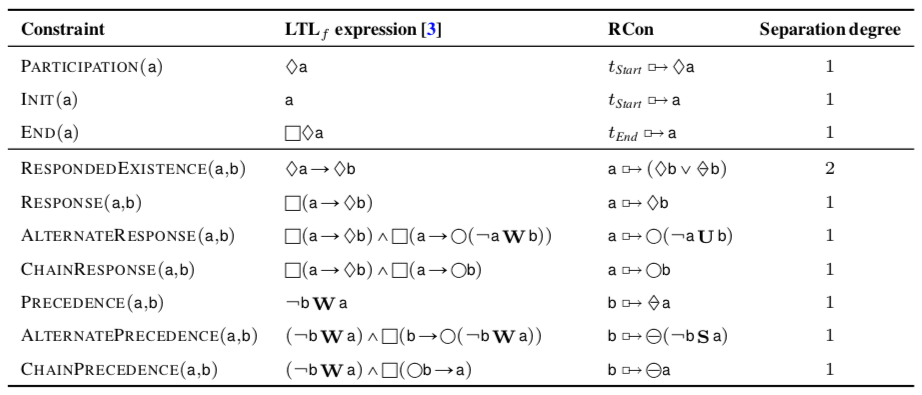
\includegraphics[width=\textwidth]{images/declare-constraints}
\caption{The most important \declare constraints expressed as \LTLf/\PLTL formulas and \emph{reactive constraints.}}
\label{fig:declare-constraints}
\end{figure}
Parameters in a template define tasks and they occurs as events in traces. In Example \ref{ex:declare-examples} we provide a glimpse of \declare patterns.
\begin{example}\label{ex:declare-examples}
Interesting \declare templates \citep{maggi2013knowledge}
\begin{itemize}
\item \textsc{Precedence}(a,b) means \emph{if b occurs then a occurs before b}.
\item \textsc{Responce}(a,b) means \emph{if a occurs then eventually b occurs after a}.
\item \textsc{ChainPrecedence}(a,b) means \emph{the occurrence of b imposes a to occur immediately before}.
\item \textsc{AlternateResponce}(a,b) means \emph{if a occurs then eventually
b occurs after a without other occurrences of a in between}.
\end{itemize}
\end{example}
In addition, one can create his own 	\declare patterns tailored for his purposes. In this way, the \declare standard template can be customized.

A given \declare constraint is verified over traces and those traces \emph{satisfy} it if they do not \emph{violate} it. Here, it is important to notice that these constraints are prone to the principle of \textit{ex falso quod libet}, namely they can be satisfied even without being activated. This represents a big issue for process mining because mining techniques might misunderstand the actual behavior of a process. The solution to this problem is to compute whether a constraint is satisfied or not only upon activation. However, we will see later how to overcome this problem in the Section \ref{sec:janus}.

Now, we give some definitions:
\begin{definition}\citep{gabbay1989declarative}\label{def:pure-temp-formula}
Given an \LTLp formula $\varphi$, we call it \emph{pure past} formula ($\varphi^\blacktriangleleft$) if it consists of only past operators; \emph{pure present} formula ($\varphi^\blacktriangledown$) if it has not any temporal operators; \emph{pure future} formula ($\varphi^\blacktriangleright$) if it consists of only future operators.
\end{definition}
\begin{example}\label{ex:pure-formulas-examples}
Pure formulas:
\begin{itemize}
\item $\boxminus(a \Rightarrow \Once b)$ is a \textbf{pure past} formula;
\item $a \Rightarrow (b \lAND c)$ is a \textbf{pure present} formula
\item $\Box(a \Rightarrow \Next b)$ is a \textbf{pure future} formula
\end{itemize}
\end{example}
The separation of an \LTLp formula to pure past/present/future formulas allows to conduct the analysis on sub-traces (i.e. one referring to the past and the other referring to the future) upon the activation. This is also known as bi-directional on-line analysis. To this extent, we rely on the Separation Theorem stated as follows:
\begin{theorem}\citep{gabbay1989declarative}\label{th:separation-theorem}
Any propositional temporal formula $\varphi$ can be rewritten as a boolean combination of pure temporal formulas.
\end{theorem}
Therefore, following Theorem \ref{th:separation-theorem}, we can give the Definition of \textit{separated formula} as follows:
\begin{definition}\citep{cecconi2018interestingness}\label{def:separated-formula}
Let  $\varphi$ an \LTLp formula over $\Sigma$. A temporal separation is a function $\S: \textsc{ltl}p_f  \rightarrow 2^{\textsc{ltl}p_f \times \textsc{ltl}p_f 	\times \textsc{ltl}p_f}$ such that: $\S(\varphi) = \{(\varphi^{\blacktriangleleft},\varphi^{\blacktriangledown},\varphi^{\blacktriangleright})_1,\dots,\\(\varphi^{\blacktriangleleft},\varphi^{\blacktriangledown},\varphi^{\blacktriangleright})_m\}$ such that:
\begin{equation}\label{eq:separated-formulas}
\varphi \equiv \bigvee^{m}_{j=1} (\varphi^{\blacktriangleleft} \lAND \varphi^{\blacktriangledown} \lAND \varphi^{\blacktriangleright})_j
\end{equation}
where $\varphi^\blacktriangleleft$, $\varphi^\blacktriangledown$ and $\varphi^\blacktriangleright$ are pure formulas over $\Sigma$ as in Definition \ref{def:pure-temp-formula}.
\end{definition}
Notice that Equation \ref{eq:separated-formulas} is a disjunction of conjunction. Moreover, each triple consisting the image function of $\S(\varphi)$ is generally called \emph{separated formula}. In the following, we give an example of separated formula.
\begin{example}\label{ex:separated-formulas}
The separated formulas for $(\Yesterday a \lOR \Diamond b$):
\begin{align*}
(\Yesterday a \lAND True \lAND True)\bigvee(True \lAND True \lAND \Diamond b)
\end{align*}
\end{example}
PUT HERE THE NEW GENERALIZATION OF THE THEOREM

Since the Janus algorithm relies on the construction of the automata for separated \LTLp formulas, we will refer to notions explained previously in Section \ref{sec:formula-to-automa}. The crucial point is that given a separated \LTLp formula $\varphi$ we can build a minimum \DFA that \emph{accepts} all and only the traces satisfying formula $\varphi$.

In the following sections, we will describe in details the Janus approach giving fundamentals definitions and theorems. Then, we will illustrate the algorithm and its practical implementation.
\section{Janus}\label{sec:janus}
Declarative process modeling defines a list of \declare constraints to be satisfied during the execution of the process model. These constraints are of a reactive nature in the sense that the occurrence of some task bounds the occurrence of other activities. As anticipated in the previous Section, this kind of behavior might lead to the principle of \textit{ex falso quod libet}, namely a constraint can be satisfied even though it is never activated. Here, the Janus approach \citep{cecconi2018interestingness} solves this problem allowing the user to indicate the activation condition for the constraint directly in the constraint formula. In this way, constraints are activated only if the activation condition holds. Therefore, we can refer to these constraints as \textit{reactive constraints} (\rcon).
\begin{definition}
Given an alphabet $\Sigma$, let $\alpha \in \Sigma$ be an \emph{activation} and $\varphi$ be an \LTLp formula over $\Sigma$. A Reactive Constraint (\rcon) $\Psi$ is a pair $(\alpha, \varphi)$, denoted as $\Psi \doteq \alpha \boxright \varphi$
\end{definition}
\subsection{Algorithm}
\section{Implementation}\label{sec:janus-implementation}
\subsection{Package Structure}
\subsection{Classes}
\section{Summary}
	\chapter{Conclusions and Future Work}\label{ch:conclusion}
Continue the introduction and possible future work
\section{Overview}
\section{Main Contributions}
\section{Future Works}
\section{Final Remarks}
	
%	\appendix 
%	\input{chapters/appendix-flloat}
%	\input{chapters/appendix-rltg}

	
	\backmatter
	\phantomsection
	
	\bibliography{bib.bib}
	

\end{document}